\begin{figure}[h]
    \centering
    \begin{minipage}[b]{0.24\textwidth}
        \centering
        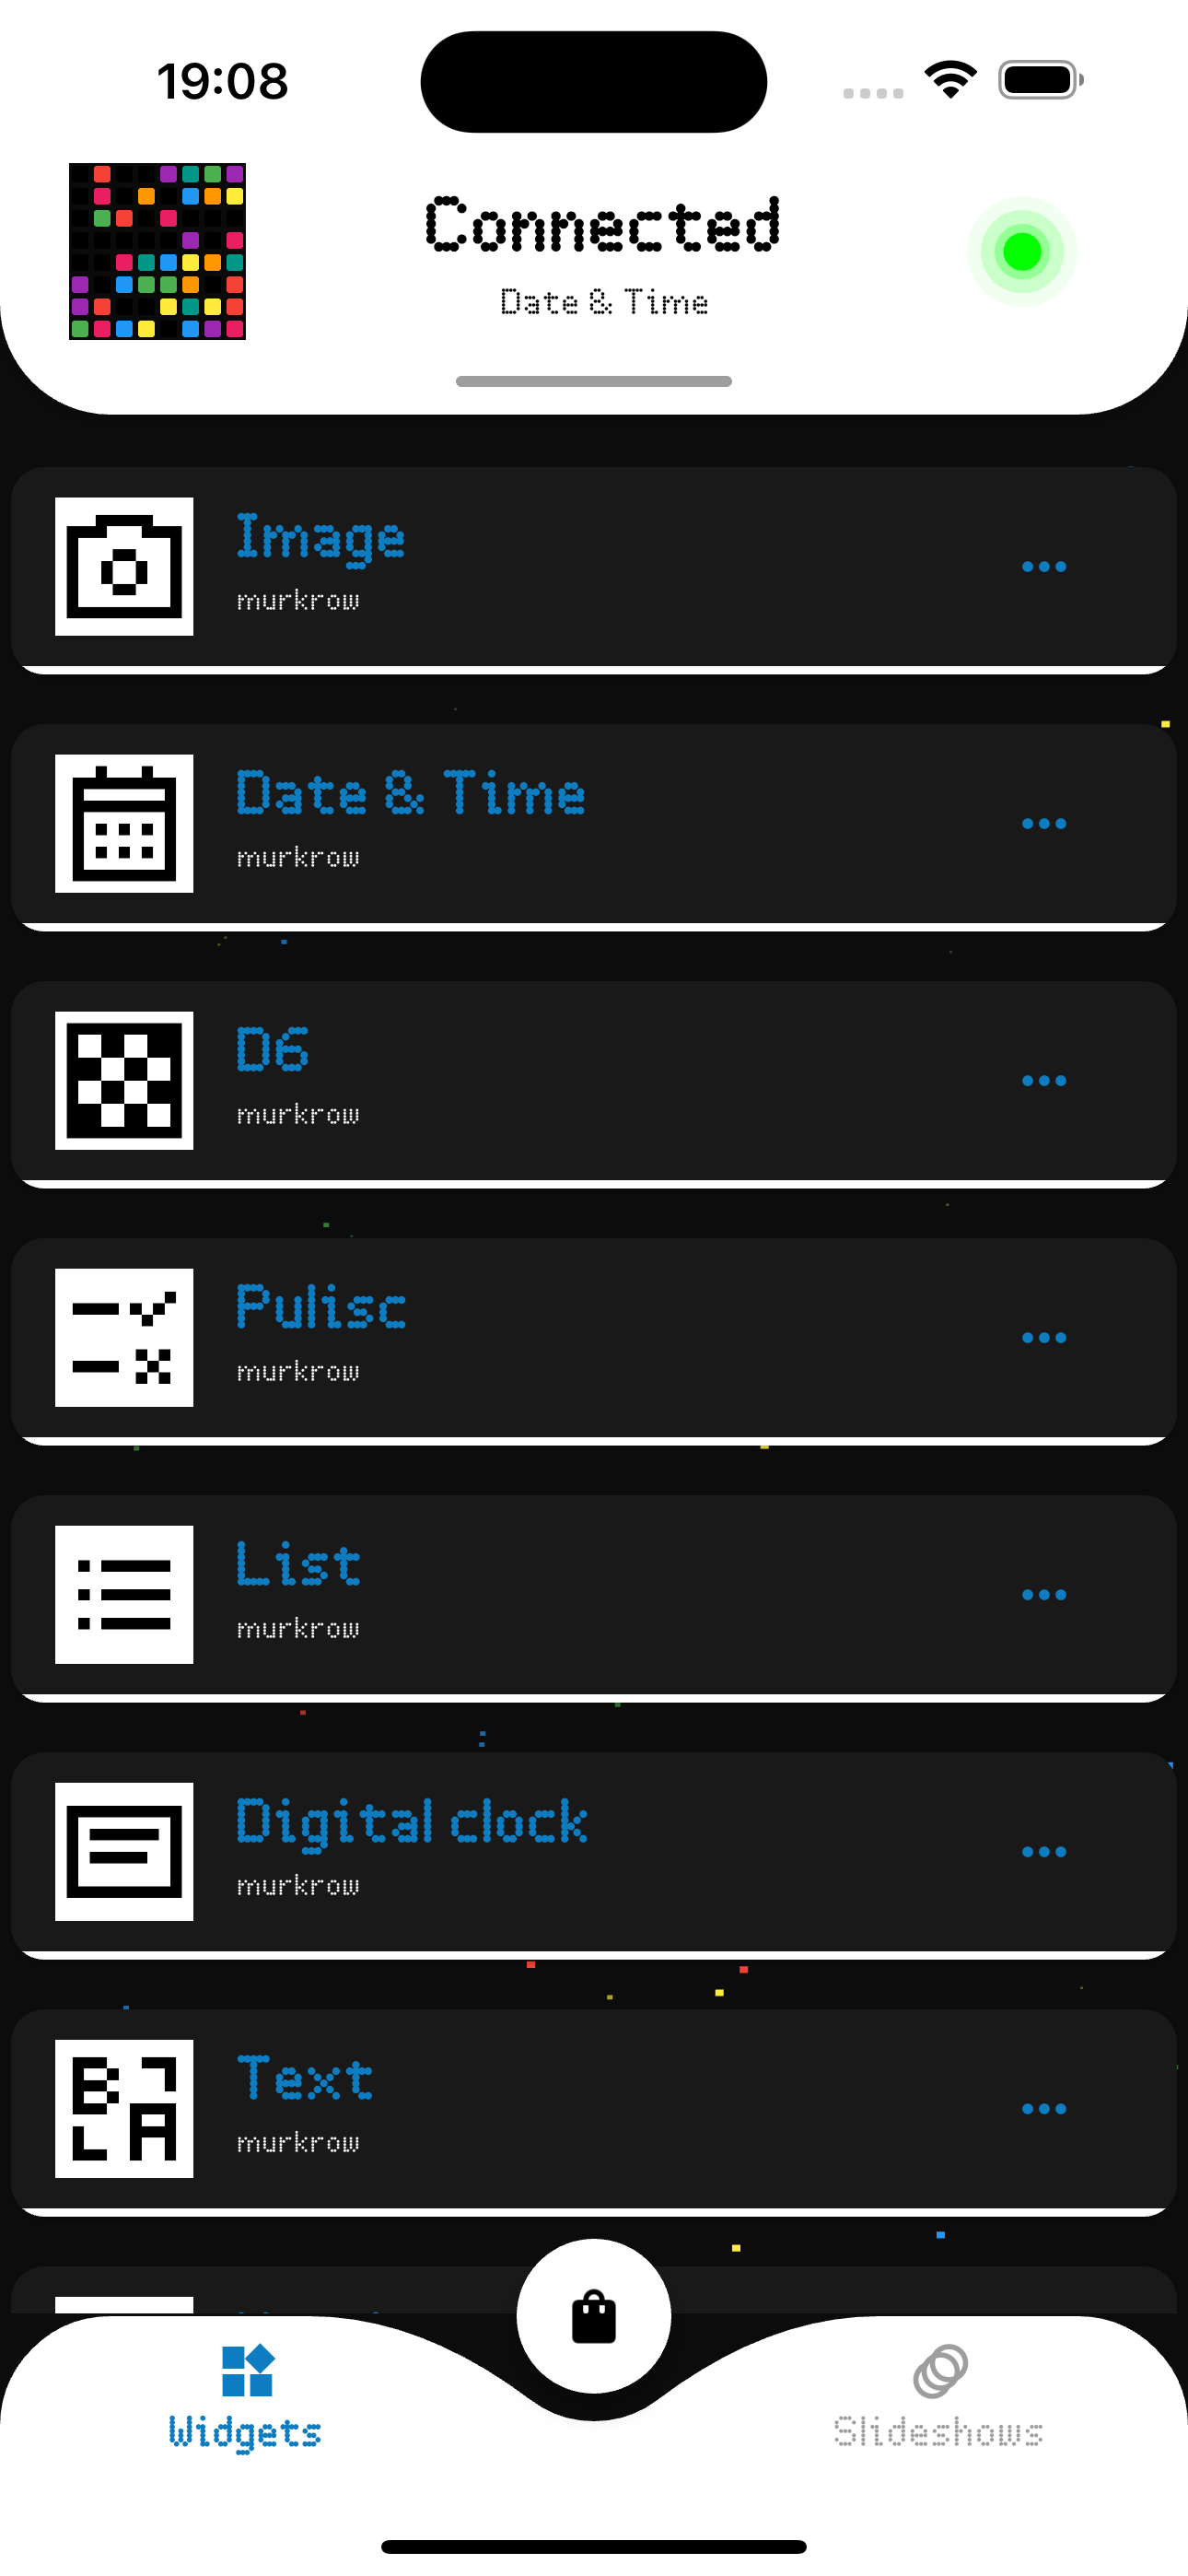
\includegraphics[width=\textwidth]{tesi/img/client_demo/installed_widgets.png}
        \caption*{Installed Widgets}
    \end{minipage}
    \begin{minipage}[b]{0.24\textwidth}
        \centering
        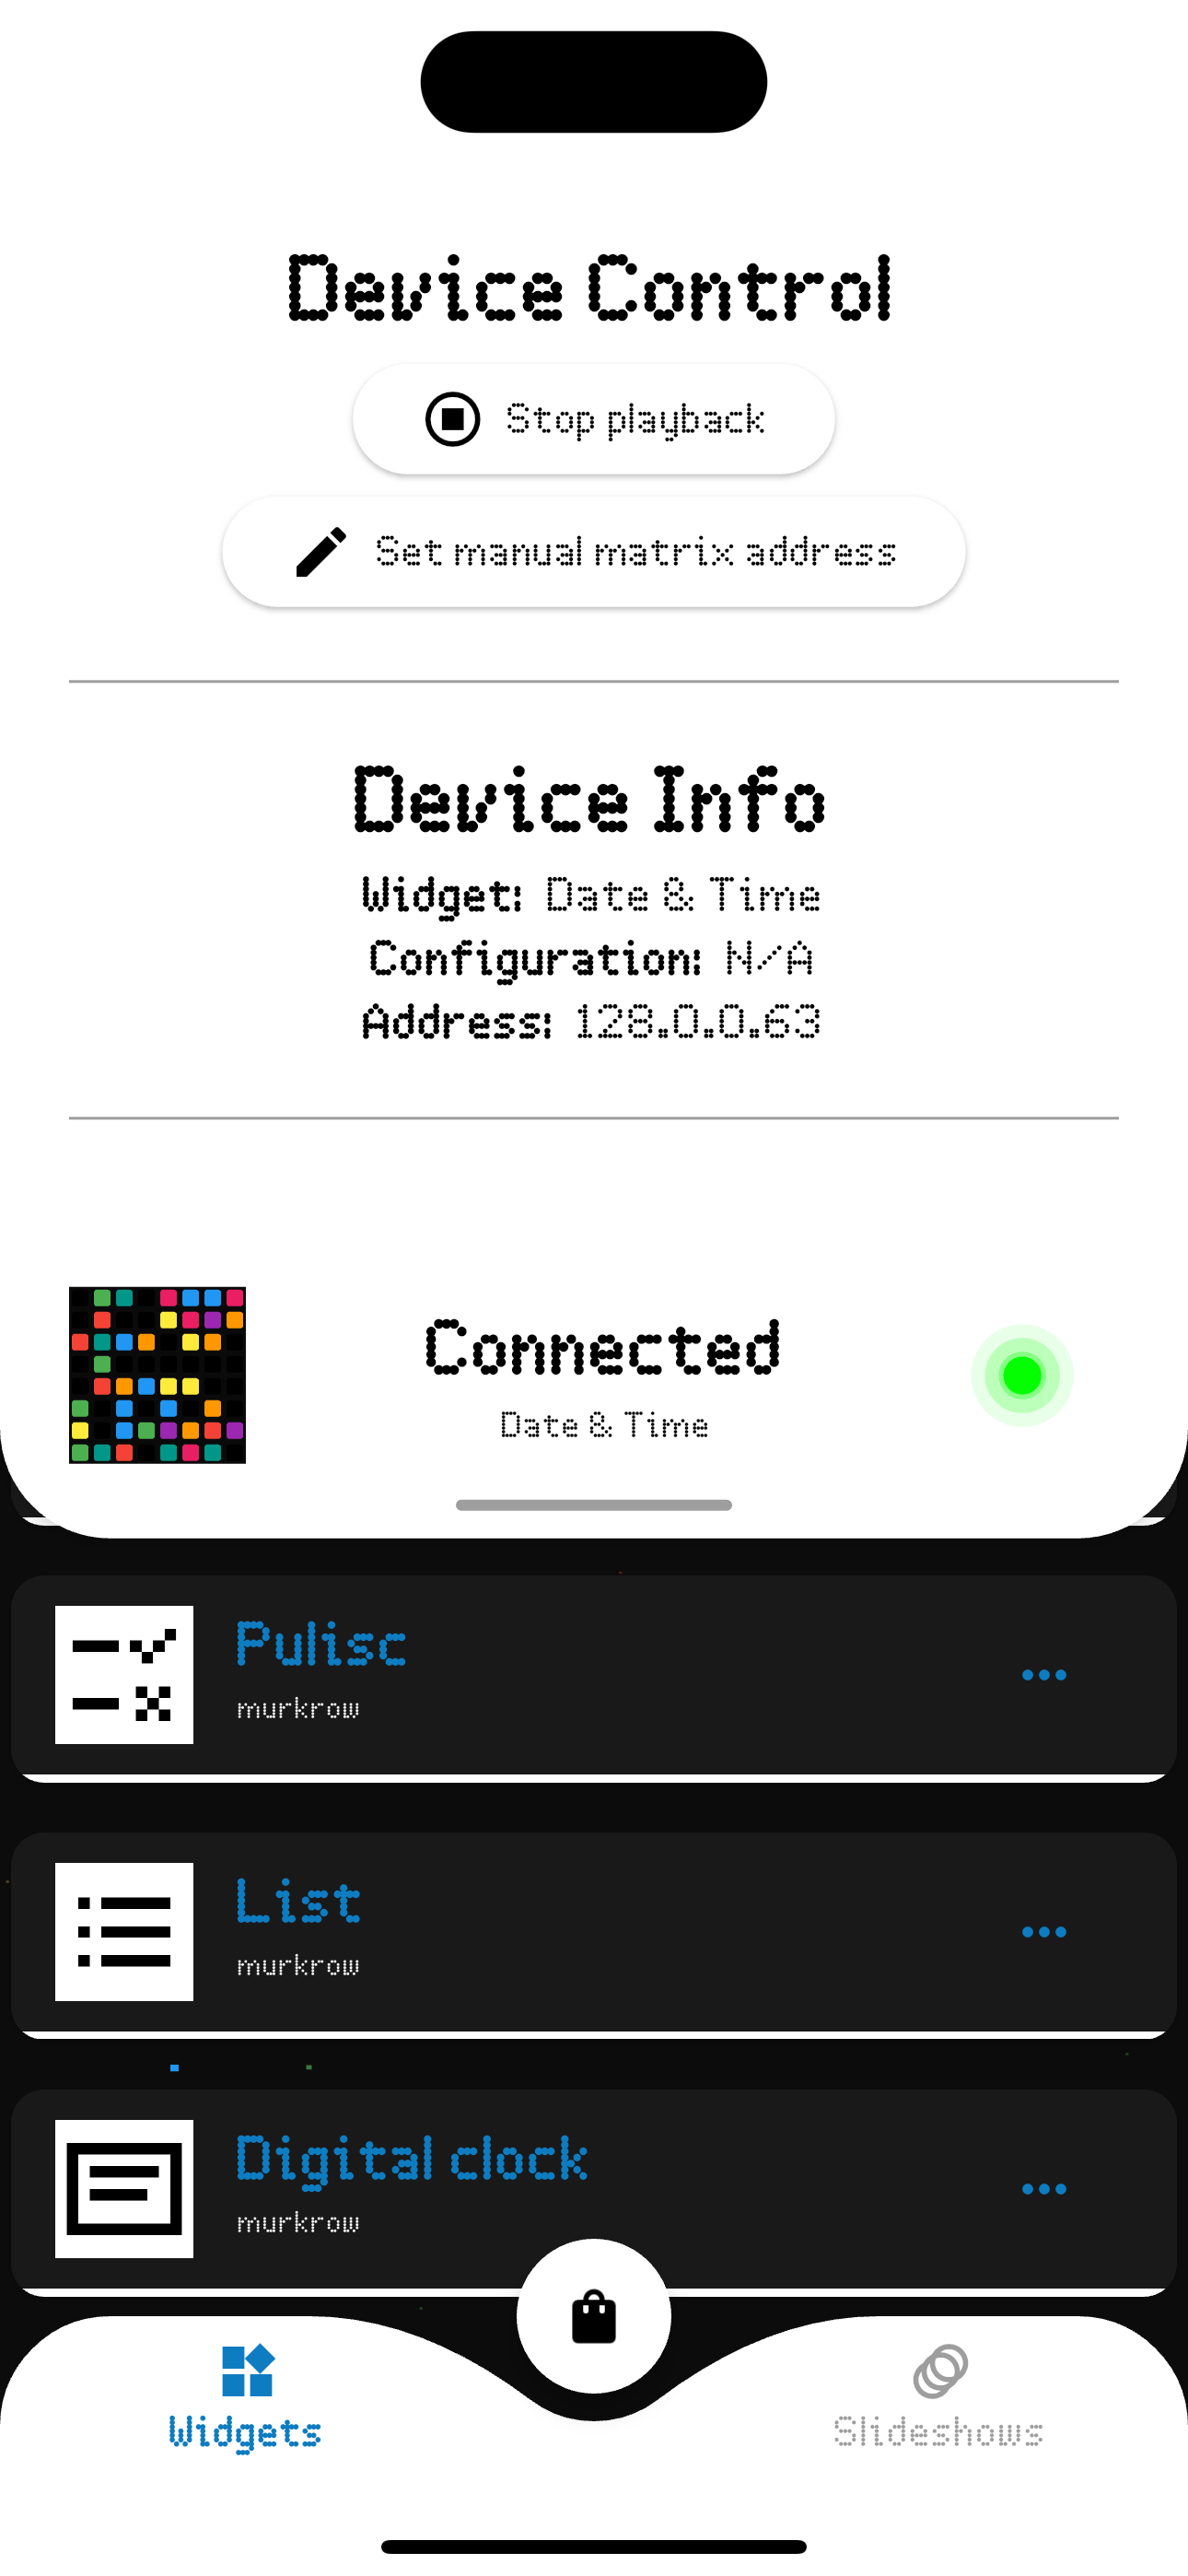
\includegraphics[width=\textwidth]{tesi/img/client_demo/matrix_control.png}
        \caption*{Matrix Control}
    \end{minipage}
    \begin{minipage}[b]{0.24\textwidth}
        \centering
        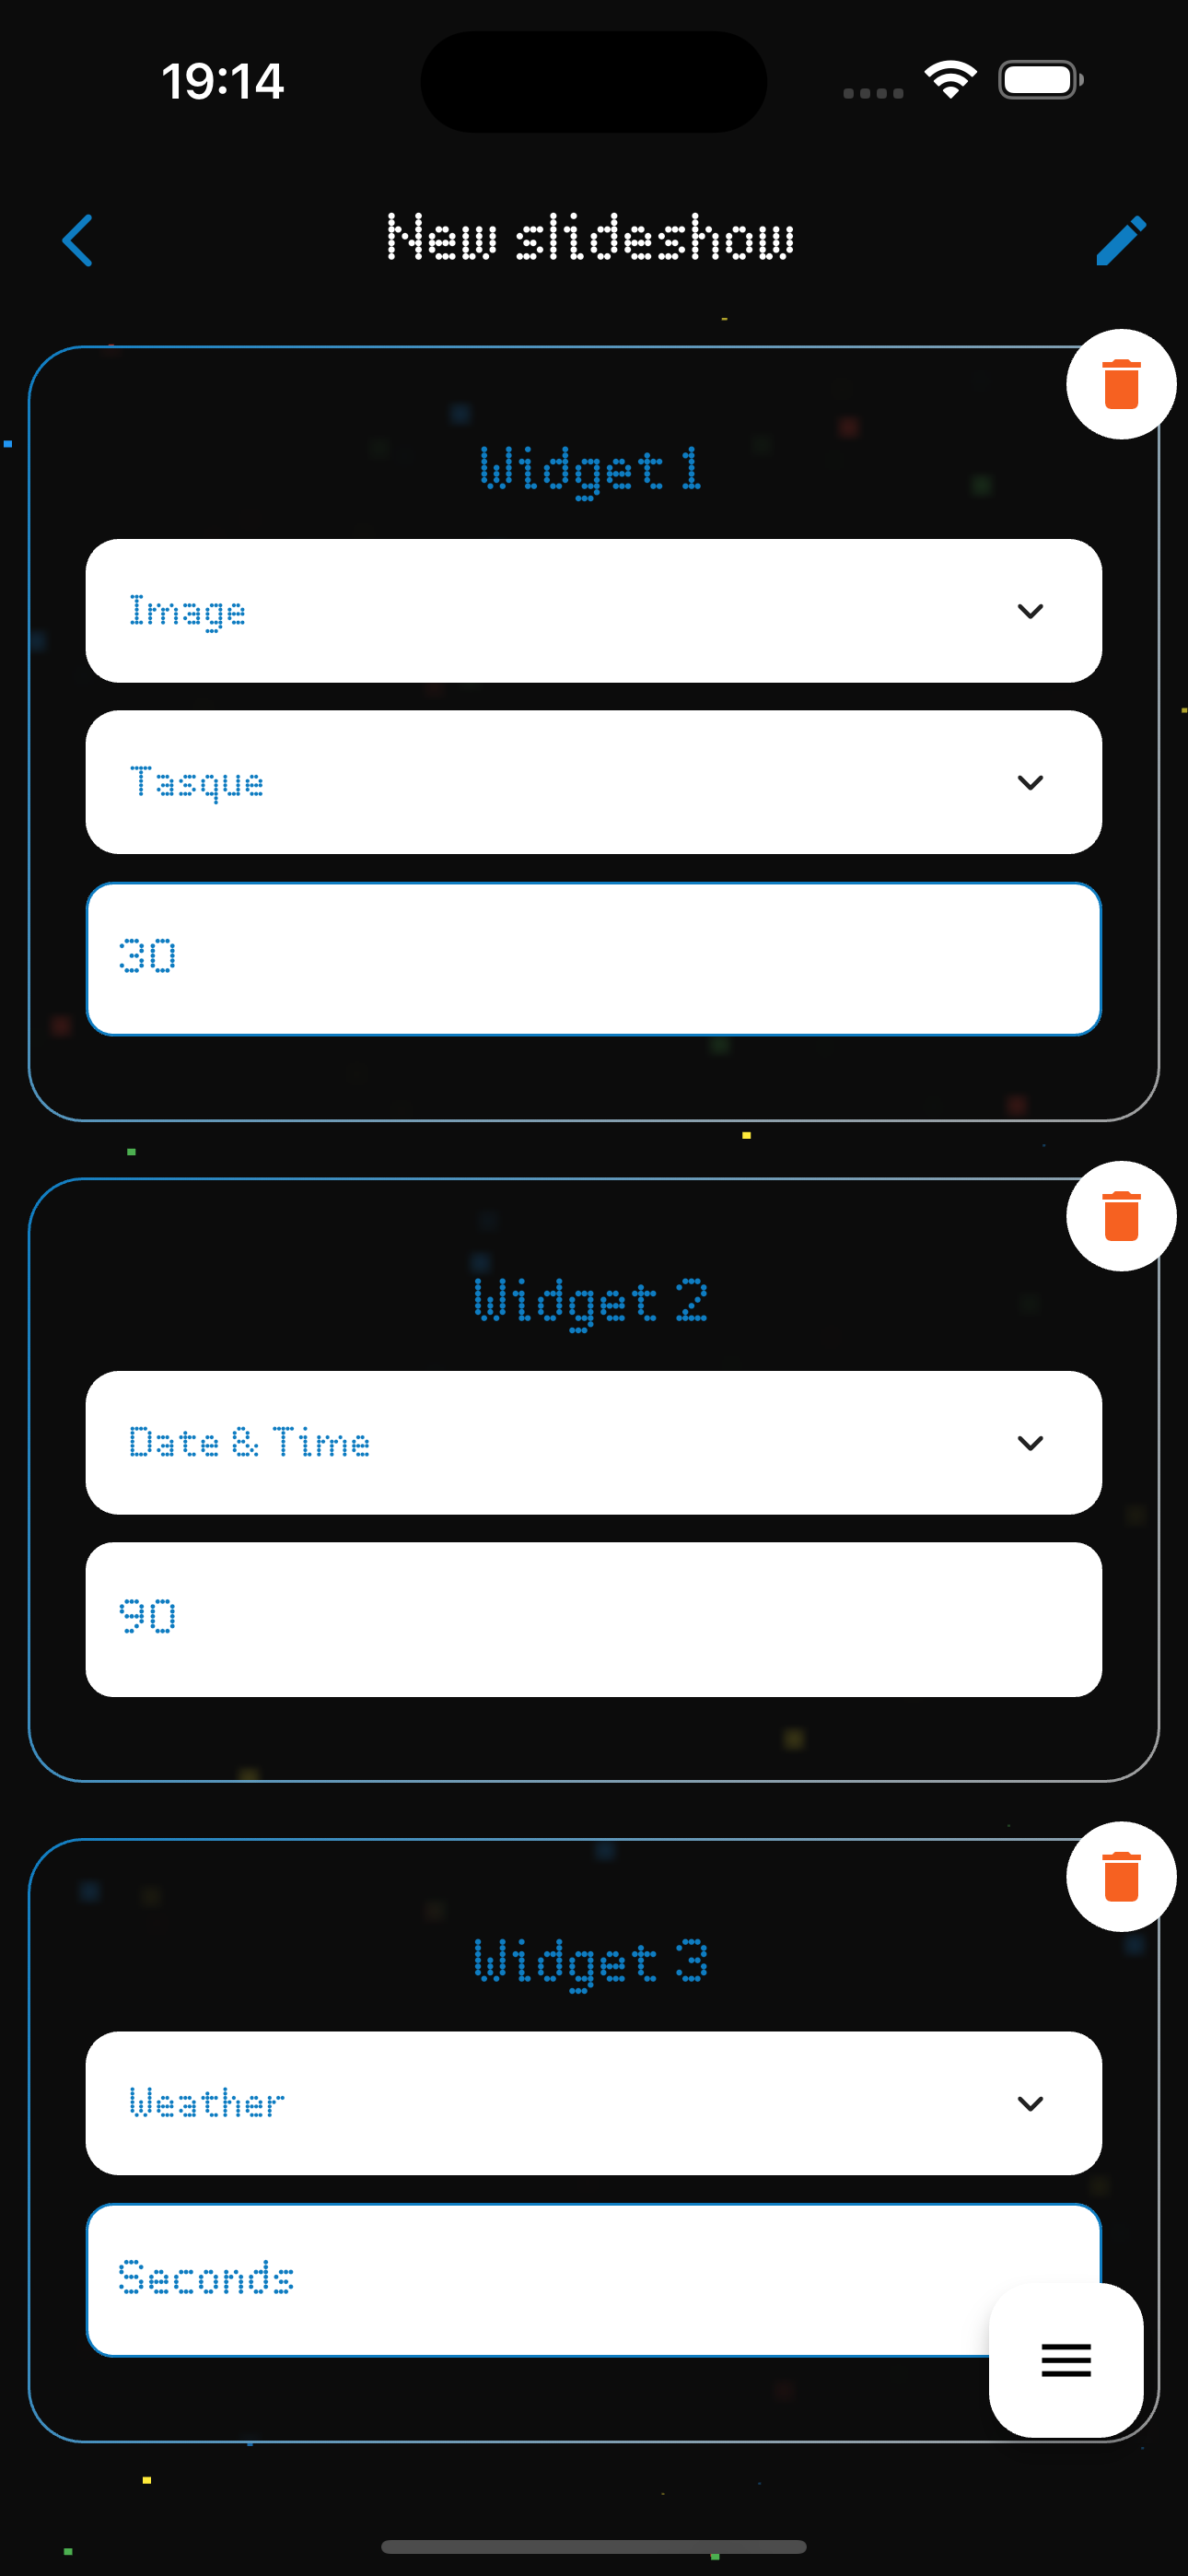
\includegraphics[width=\textwidth]{tesi/img/client_demo/slideshows.png}
        \caption*{Slideshow Editor}
    \end{minipage}
    \begin{minipage}[b]{0.24\textwidth}
        \centering
        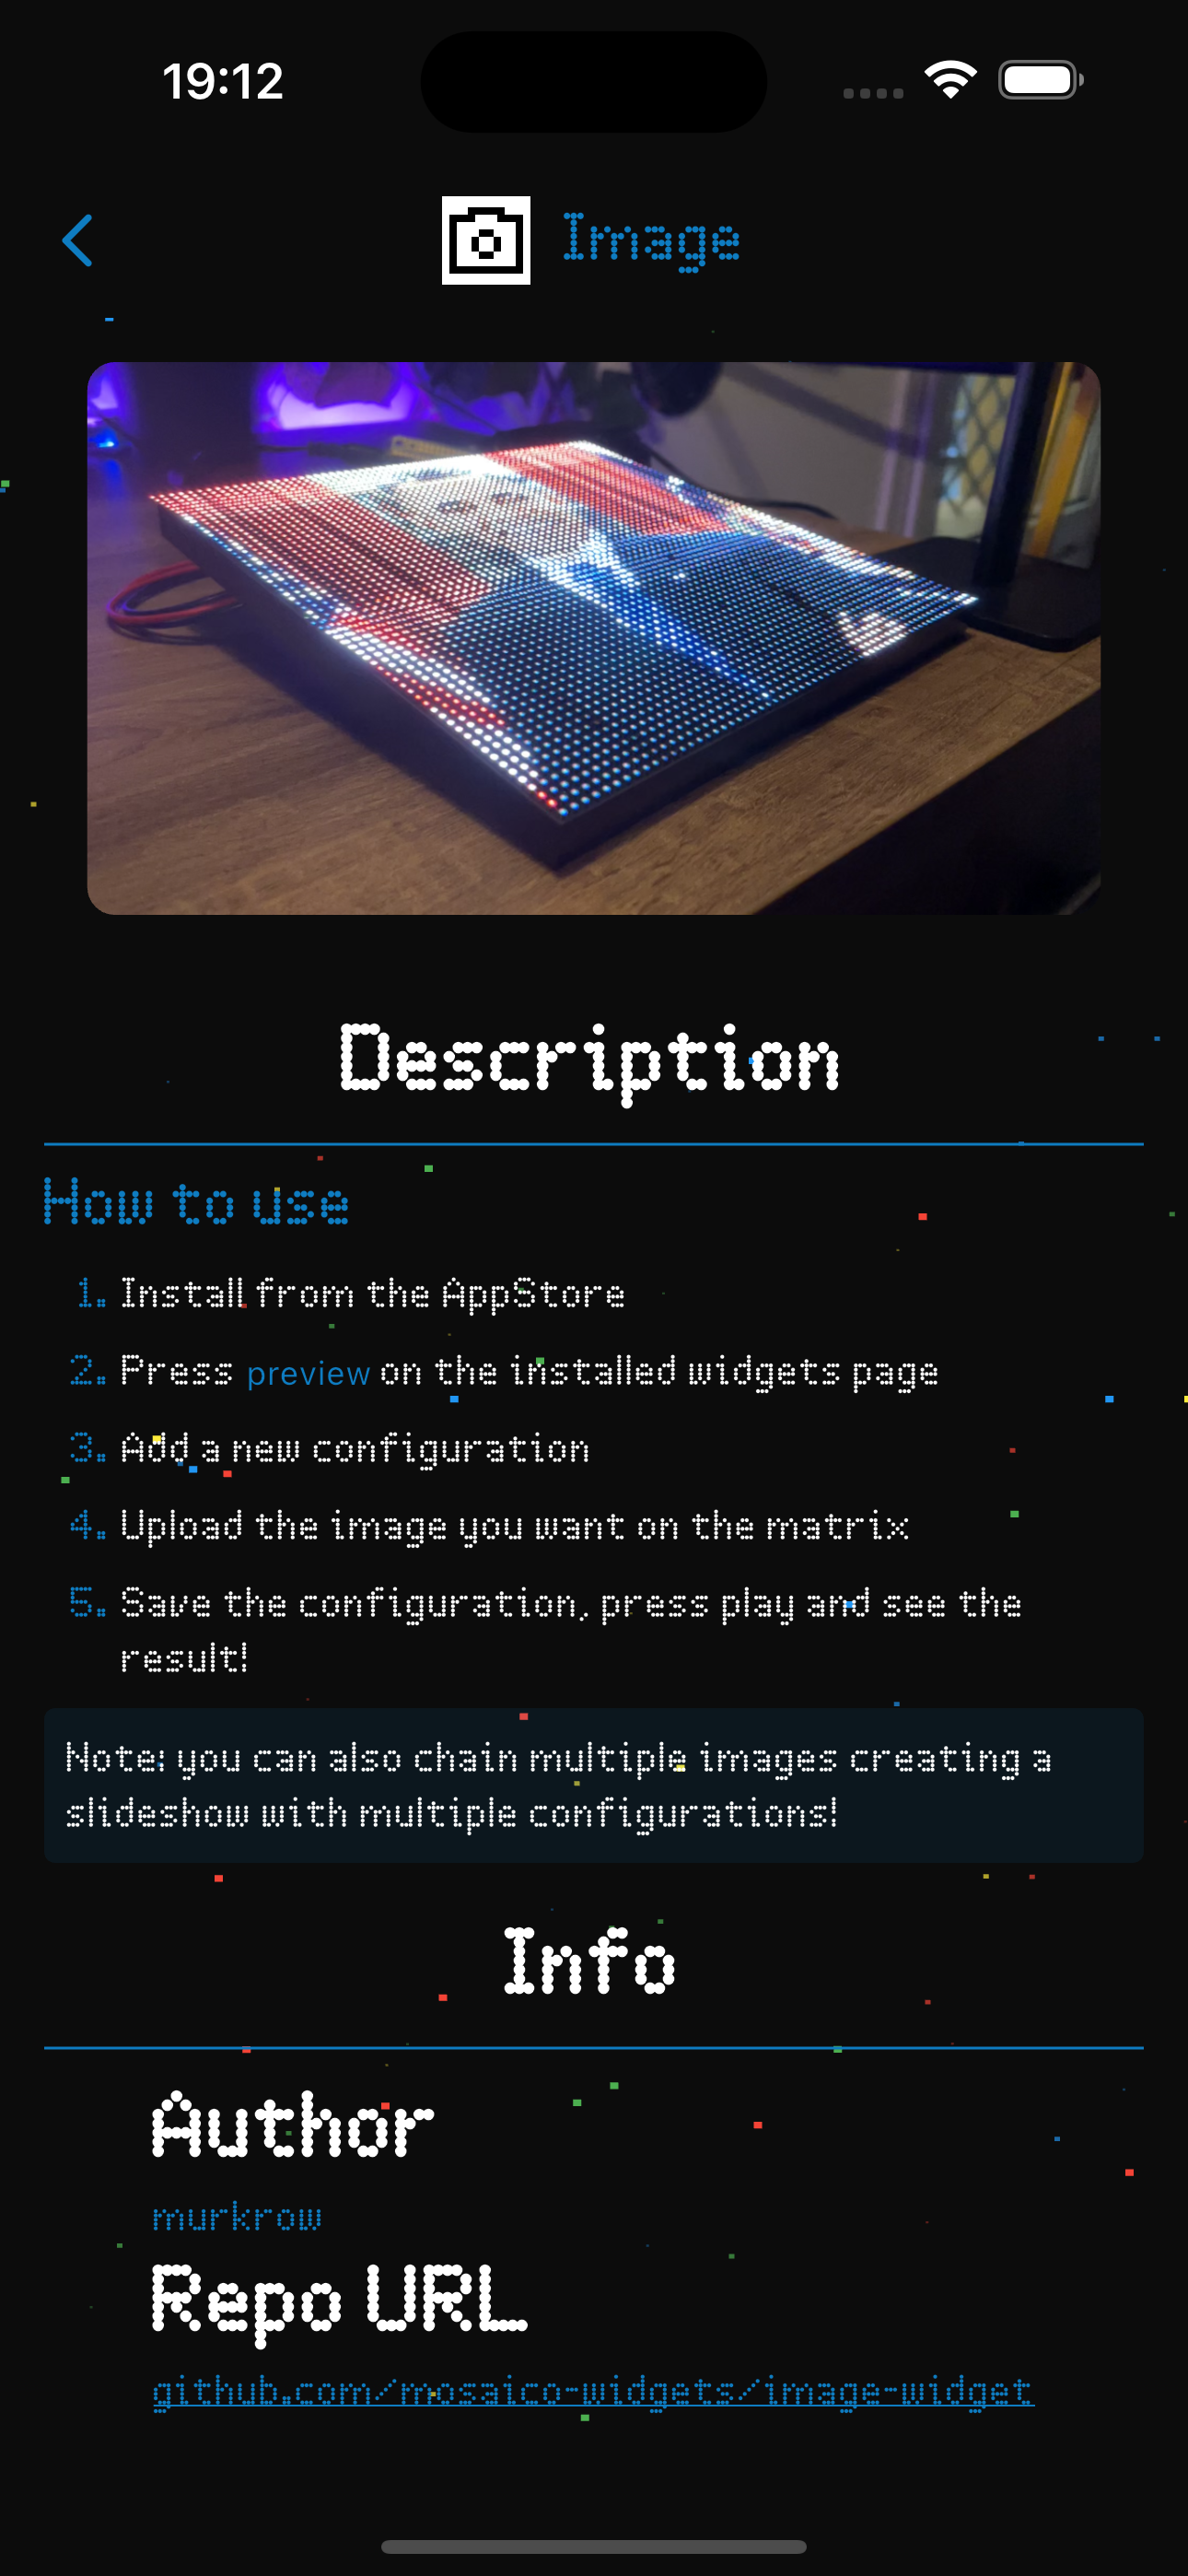
\includegraphics[width=\textwidth]{tesi/img/client_demo/store.png}
        \caption*{Widget Store}
    \end{minipage}
\end{figure}

Creating a companion client for my project was a relatively straightforward task, given my extensive experience as a mobile app developer. However, the distinctive element of this particular app is the use of the Flutter framework. Having worked with both native and web development technologies, I was intrigued by Flutter’s potential, especially since it is a well-regarded, Google-supported framework designed for cross-platform development. Flutter allows developers to create applications for various platforms with minimal additional effort, using a single codebase.

\newpage

\section{Showcase}
\subsection{Home}
Upon launching the application, the user is greeted by a tabbed interface that divides the app into two primary sections: the Installed Widgets page and the Slideshows page. A floating action button located at the center of the bottom navigation bar changes its function depending on the active tab. When viewing the Installed Widgets page, the button displays a shopping bag icon, which opens the widget store when clicked. On the Slideshows page, the button instead shows a "plus" icon, which initiates the creation of a new slideshow.

\begin{figure}[h]
    \centering
    \begin{minipage}[b]{0.45\textwidth}
        \centering
        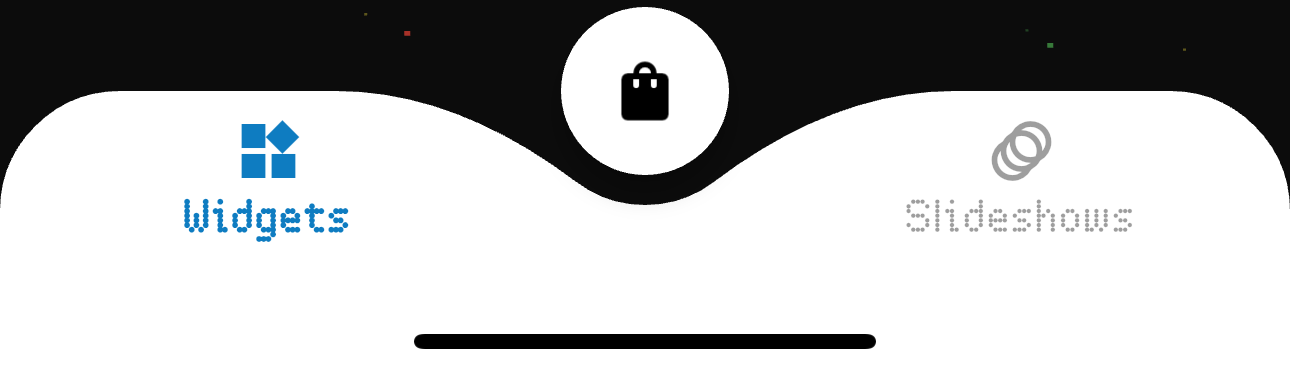
\includegraphics[width=\textwidth]{tesi/img/tab_bar/tab-bar-widgets.png}
        \caption*{Widgets Tab}
    \end{minipage}
    \begin{minipage}[b]{0.45\textwidth}
        \centering
        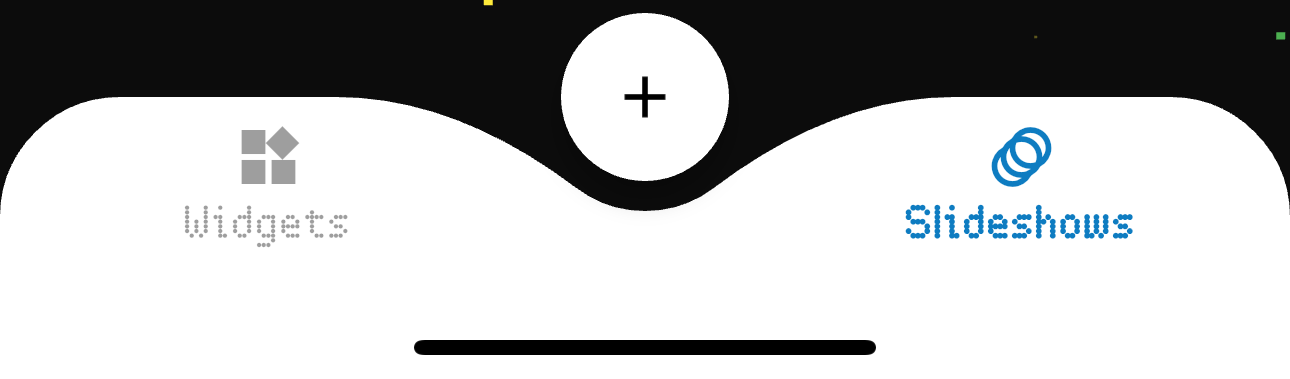
\includegraphics[width=\textwidth]{tesi/img/tab_bar/tab-bar-slideshows.png}
        \caption*{Slideshows Tab}
    \end{minipage}
\end{figure}

\subsection{Matrix Control}
At the top of the screen, a sliding panel displays essential information such as the connection status and the currently active widget. Pulling the panel down reveals further details about the matrix connection, including additional configuration options. Users can perform actions such as stopping playback or manually inputting the matrix's address.

\begin{figure}[h]
    \centering
    \begin{minipage}[b]{0.32\textwidth}
        \centering
        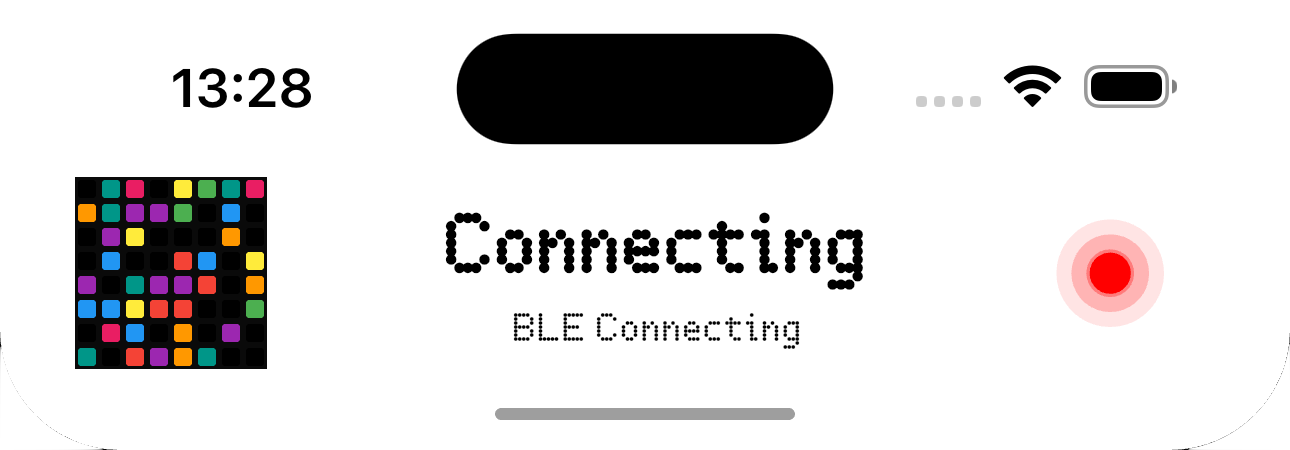
\includegraphics[width=\textwidth]{tesi/img/matrix_status_notch/connecting.png}
        \caption*{Connecting to Matrix}
    \end{minipage}
    \begin{minipage}[b]{0.32\textwidth}
        \centering
        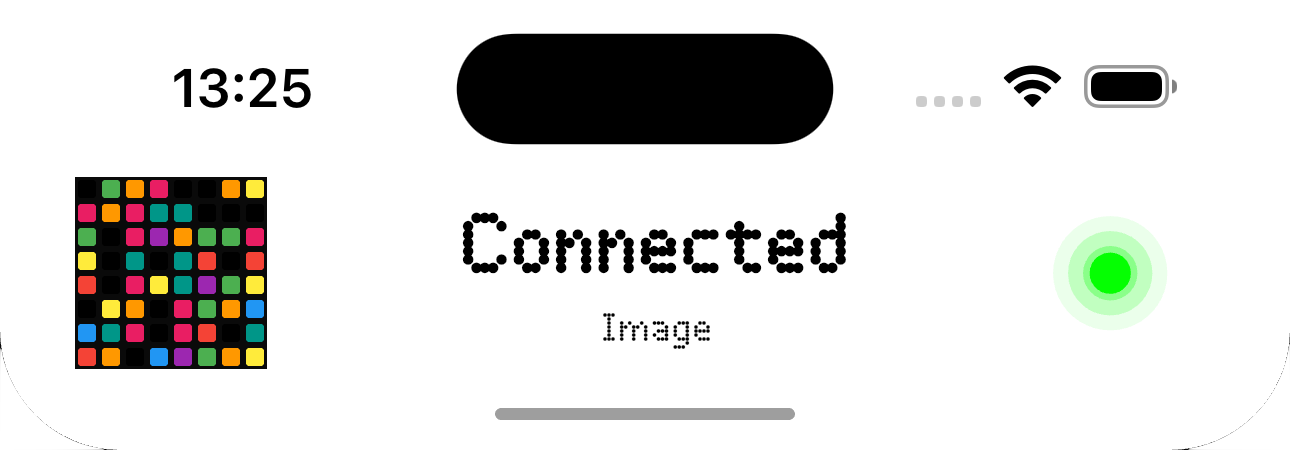
\includegraphics[width=\textwidth]{tesi/img/matrix_status_notch/connected.png}
        \caption*{Matrix Connected}
    \end{minipage}
    \begin{minipage}[b]{0.32\textwidth}
        \centering
        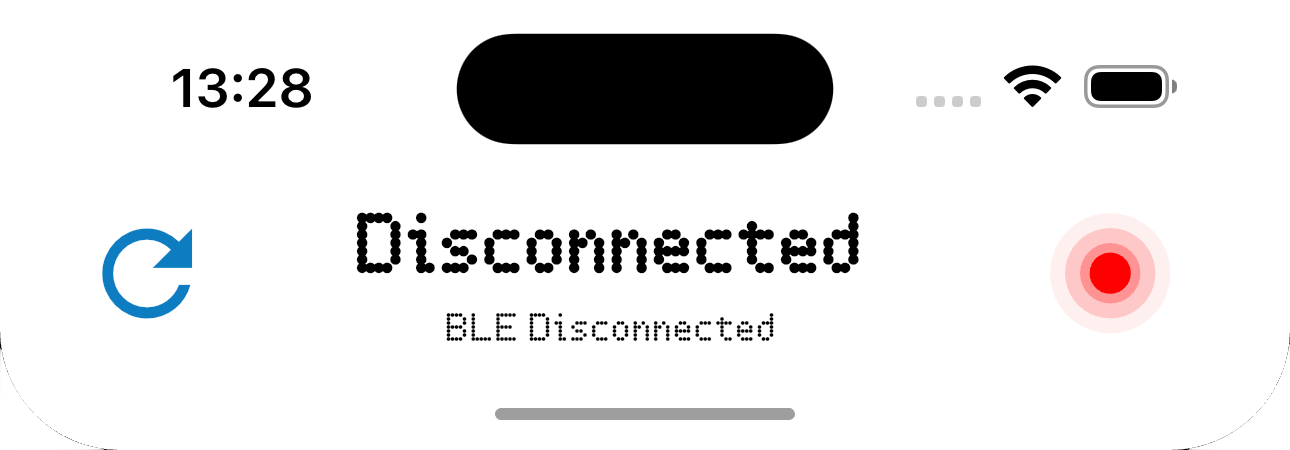
\includegraphics[width=\textwidth]{tesi/img/matrix_status_notch/disconnected.png}
        \caption*{Matrix Not Reachable}
    \end{minipage}
\end{figure}

\newpage

\subsection{Installed Widgets}
This is the default screen presented when the app launches. It lists all the widgets currently installed on the matrix, which have been downloaded from the store. Users can activate a widget by simply tapping on it. If the widget does not require further configuration, it will be displayed immediately on the matrix. However, if it is configurable, a configuration selector will prompt the user to choose a specific configuration before activating the widget.

\begin{figure}[h]
    \centering
    \begin{minipage}[b]{0.32\textwidth}
        \centering
        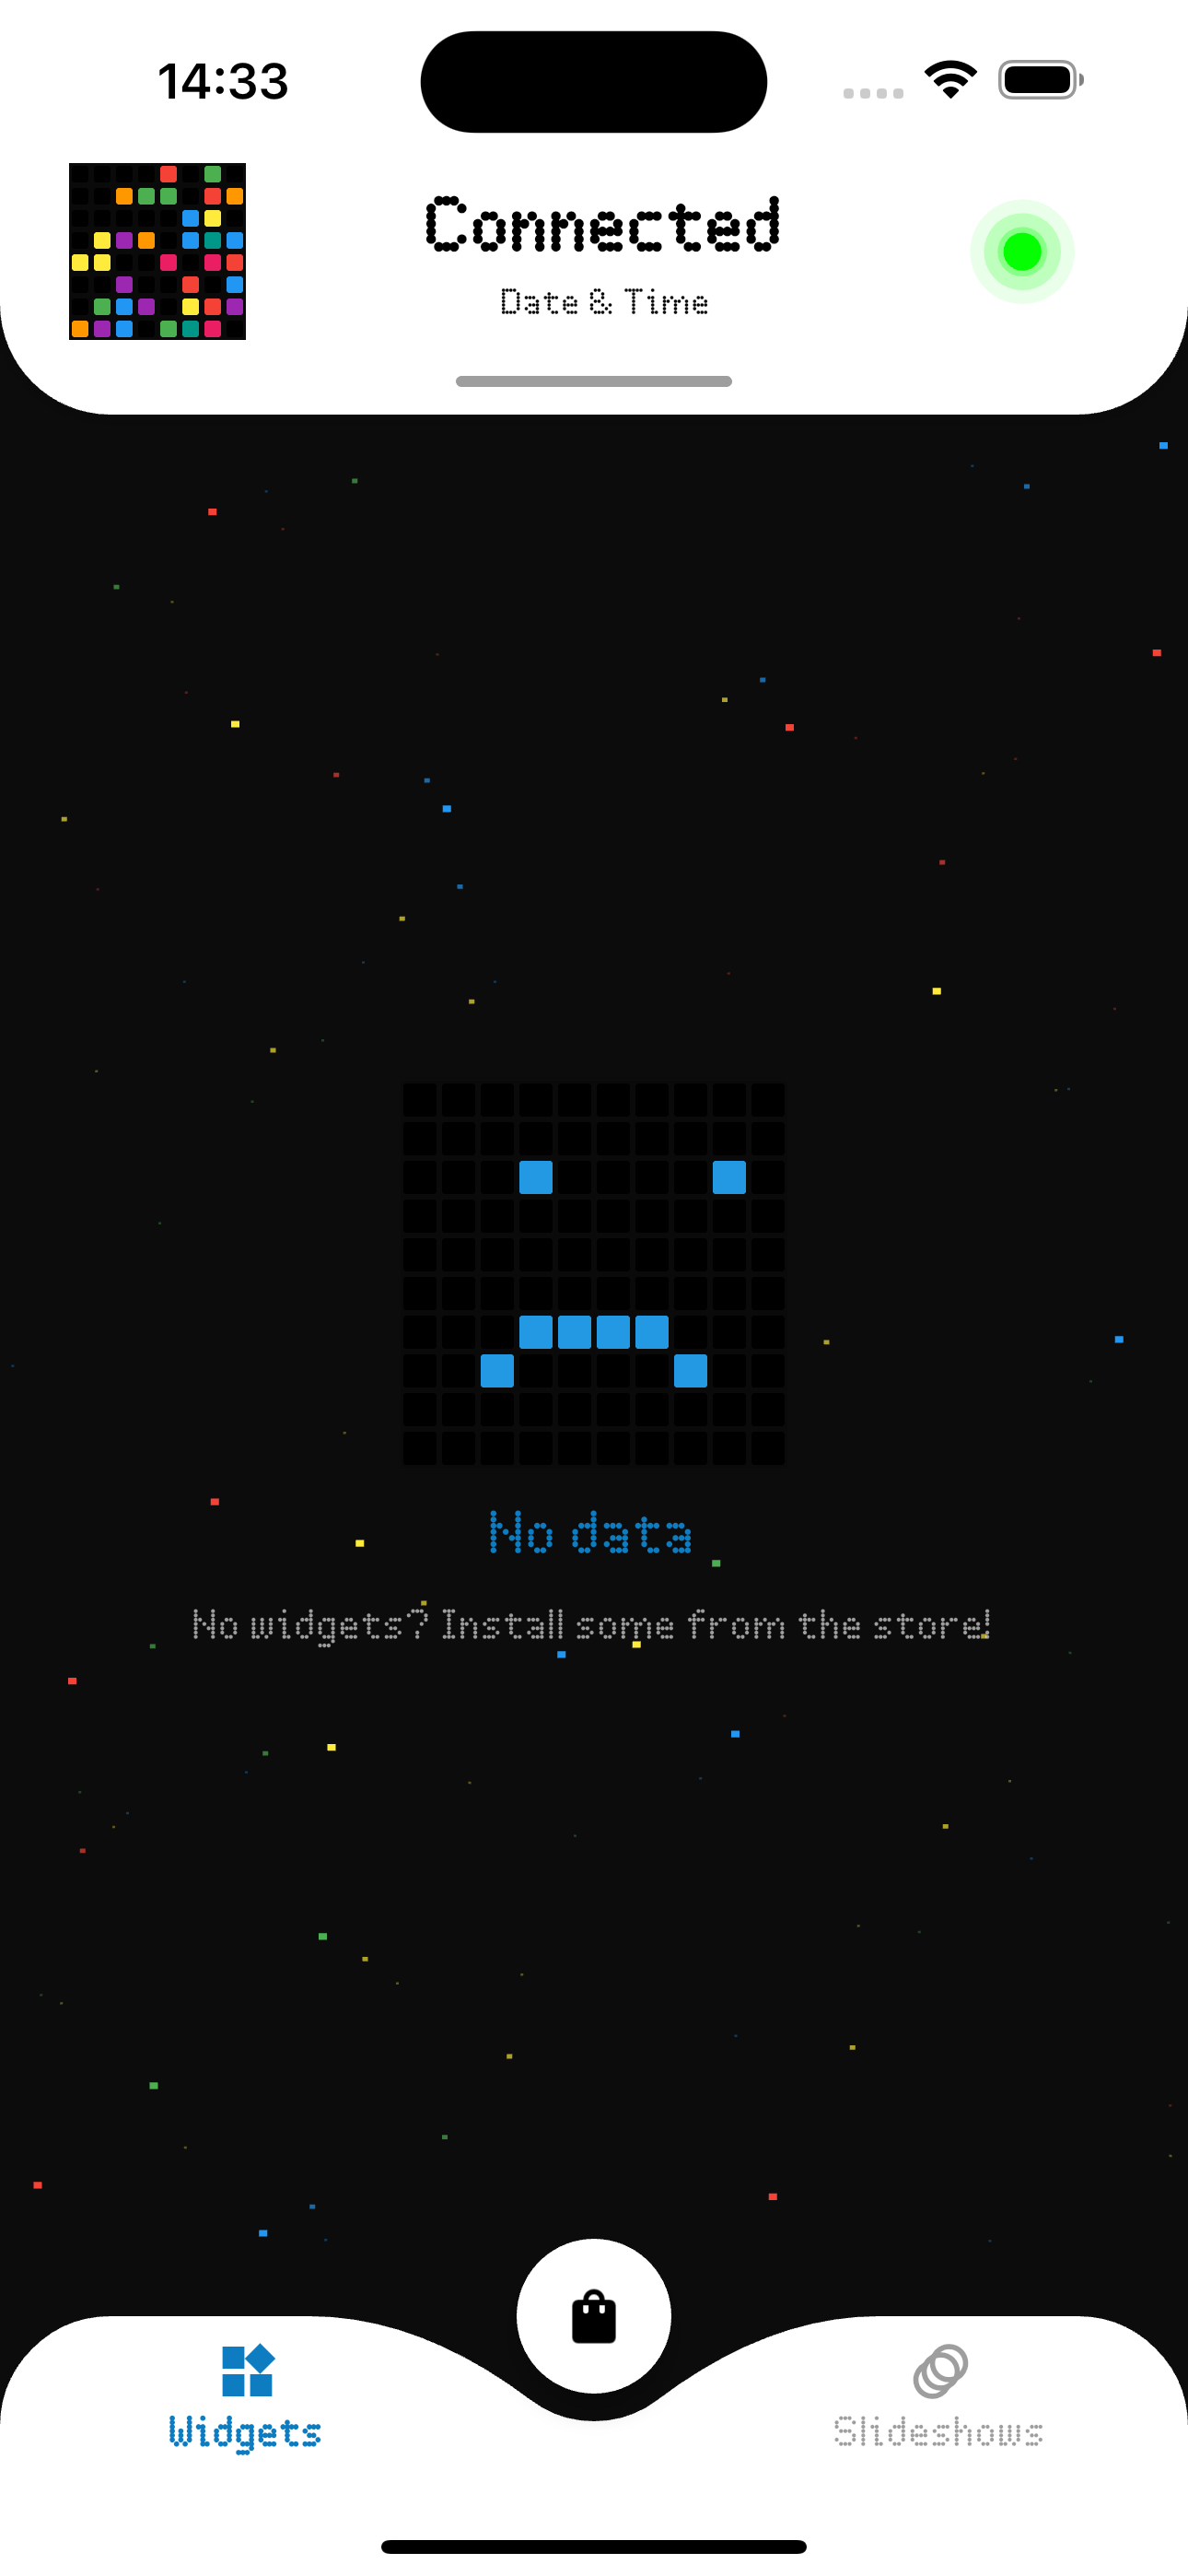
\includegraphics[width=\textwidth]{tesi/img/client_demo/installed_widgets/no_data.png}
        \caption*{No Widgets Installed}
    \end{minipage}
    \begin{minipage}[b]{0.32\textwidth}
        \centering
        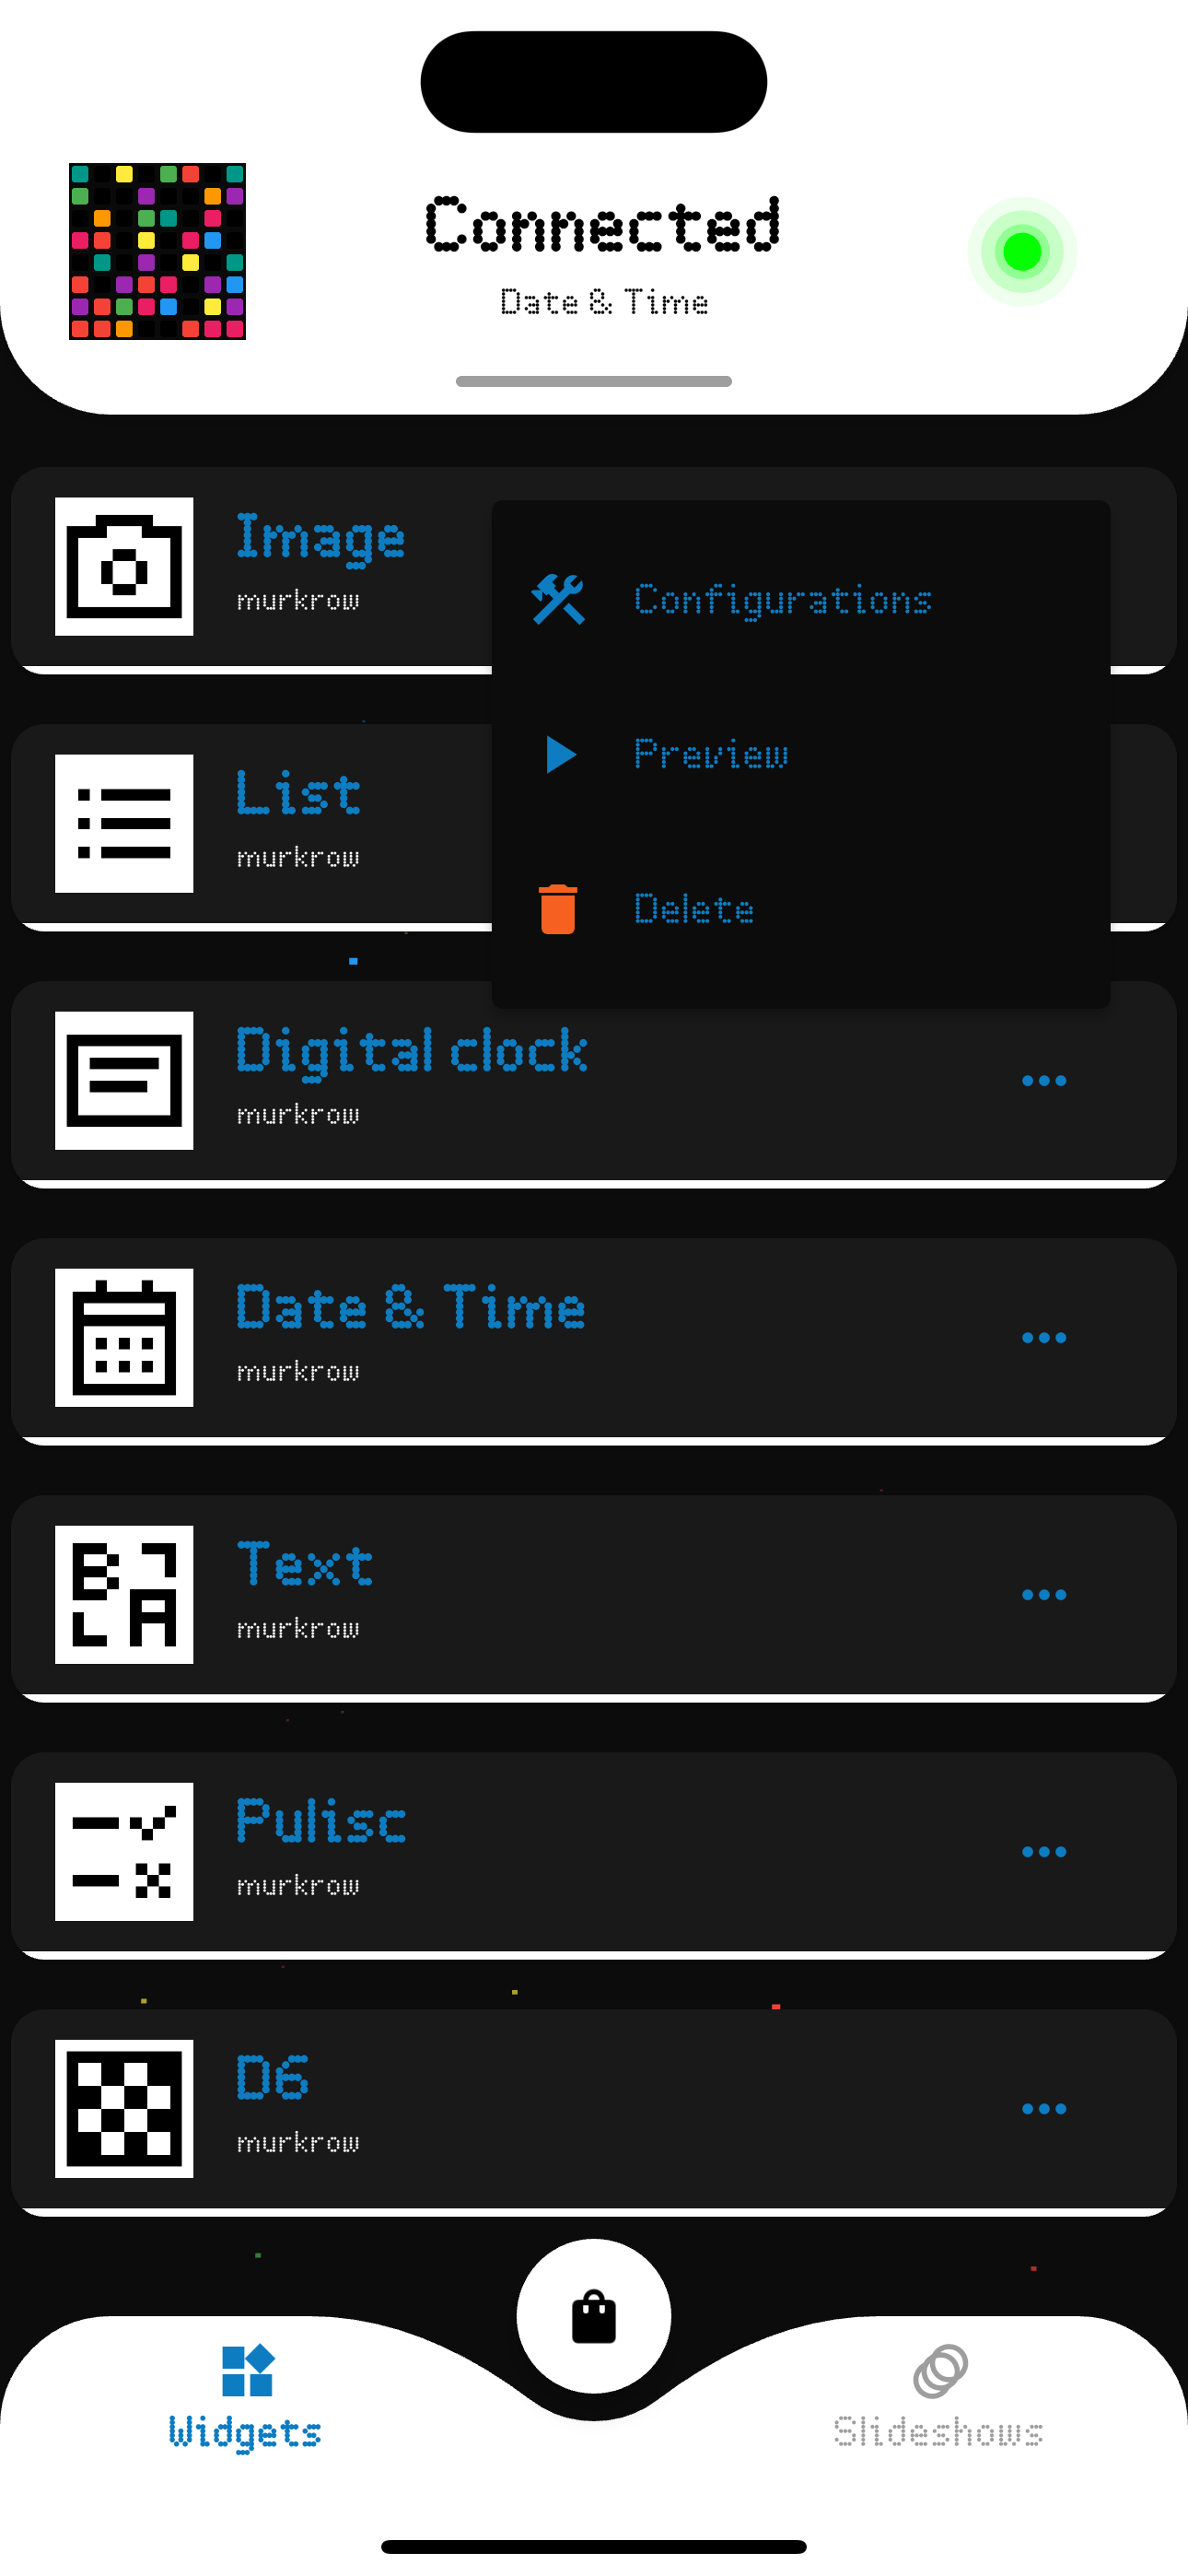
\includegraphics[width=\textwidth]{tesi/img/client_demo/installed_widgets/page.png}
        \caption*{Installed Widget Actions}
    \end{minipage}
    \begin{minipage}[b]{0.32\textwidth}
        \centering
        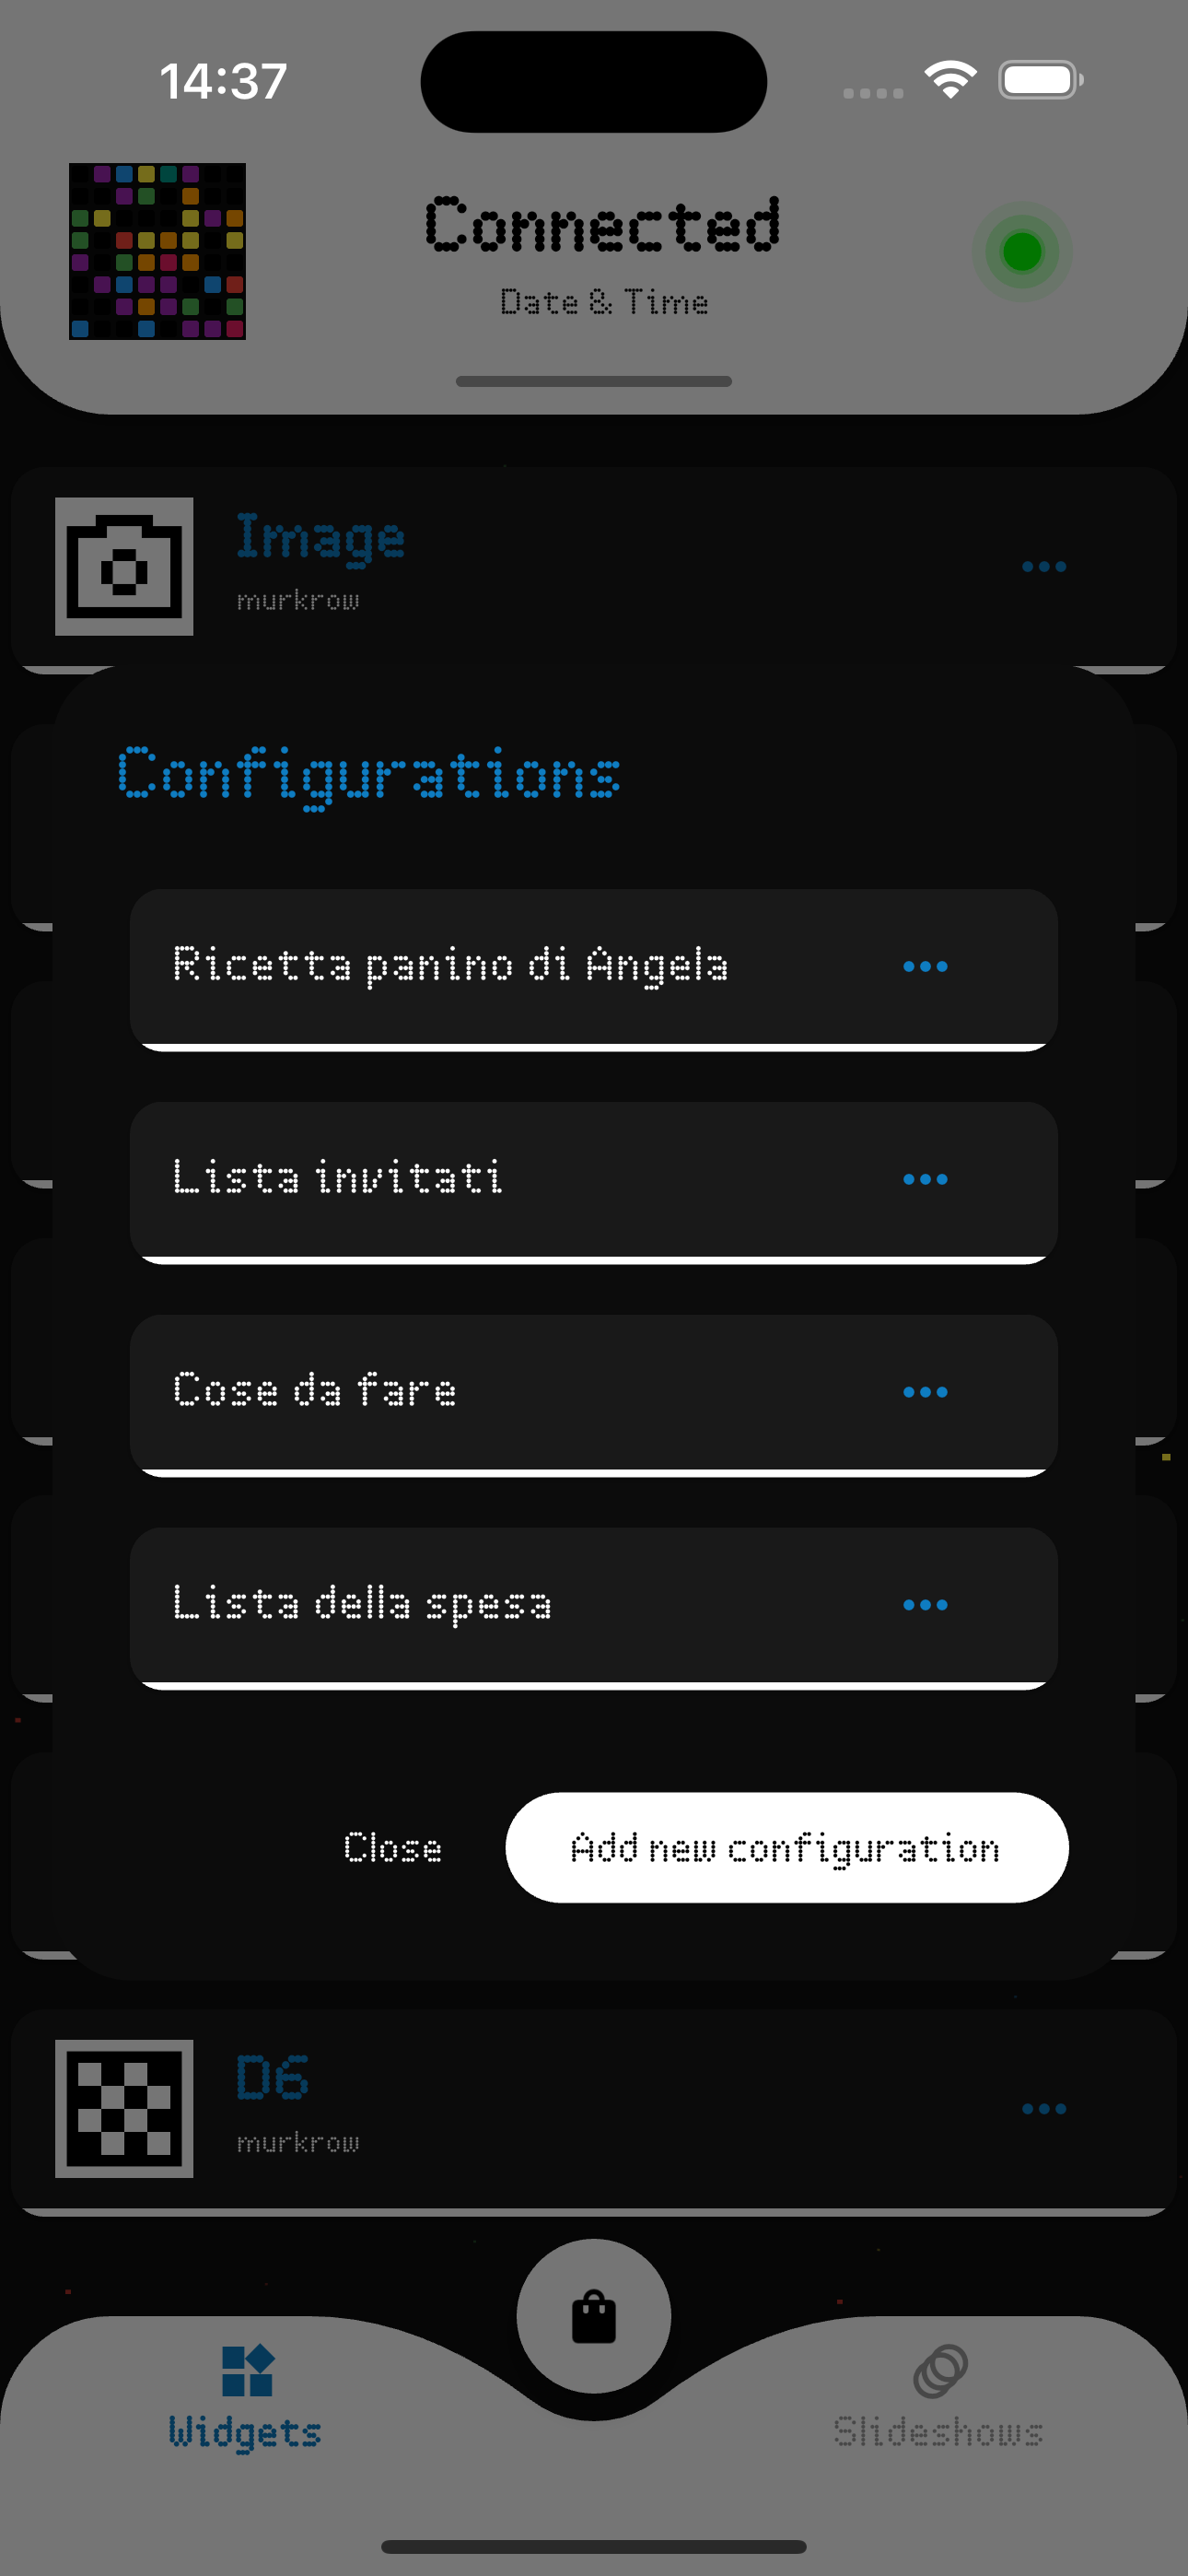
\includegraphics[width=\textwidth]{tesi/img/client_demo/installed_widgets/config_choice.png}
        \caption*{Configuration Selector}
    \end{minipage}
\end{figure}
\newpage
\subsection{Widget Store}
The widget store provides users with a space to discover new widgets. A main page lists all available widgets, each represented by a tile. By clicking on a tile, users can view more detailed information about the widget, including an image carousel, a rich markdown description, and details about the widget’s author and source code. Notably, all widgets in the store must be uploaded to a publicly accessible repository, ensuring that the ecosystem remains entirely open-source.

\begin{figure}[h]
    \centering
    \begin{minipage}[b]{0.32\textwidth}
        \centering
        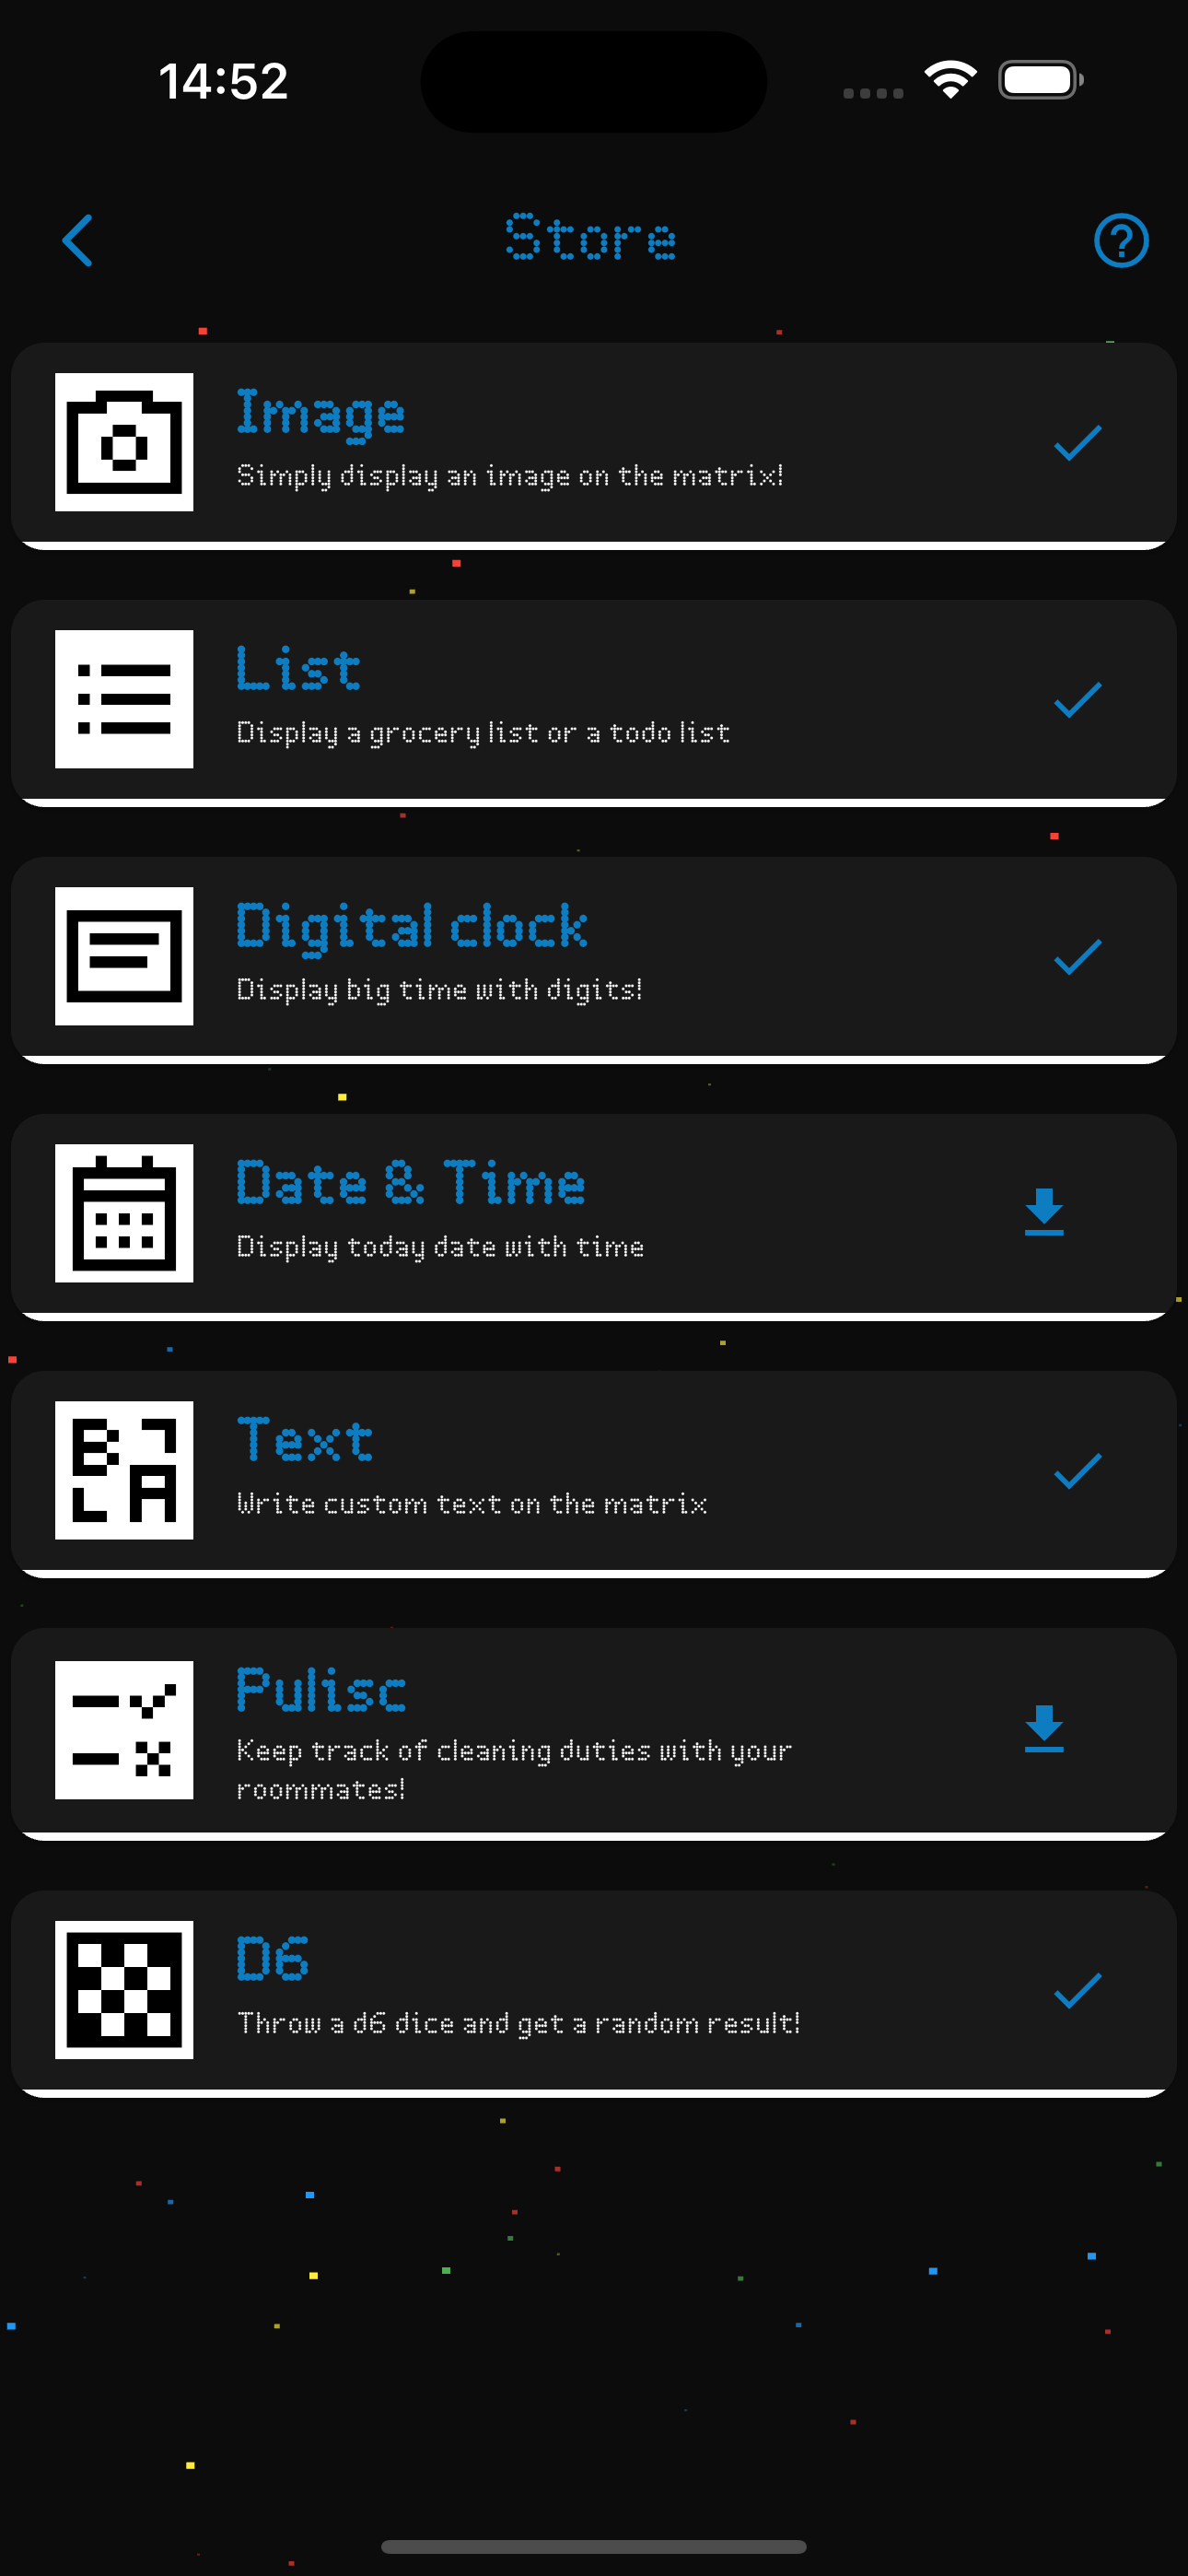
\includegraphics[width=\textwidth]{tesi/img/client_demo/store/page.png}
        \caption*{Store Overview}
    \end{minipage}
    \begin{minipage}[b]{0.32\textwidth}
        \centering
        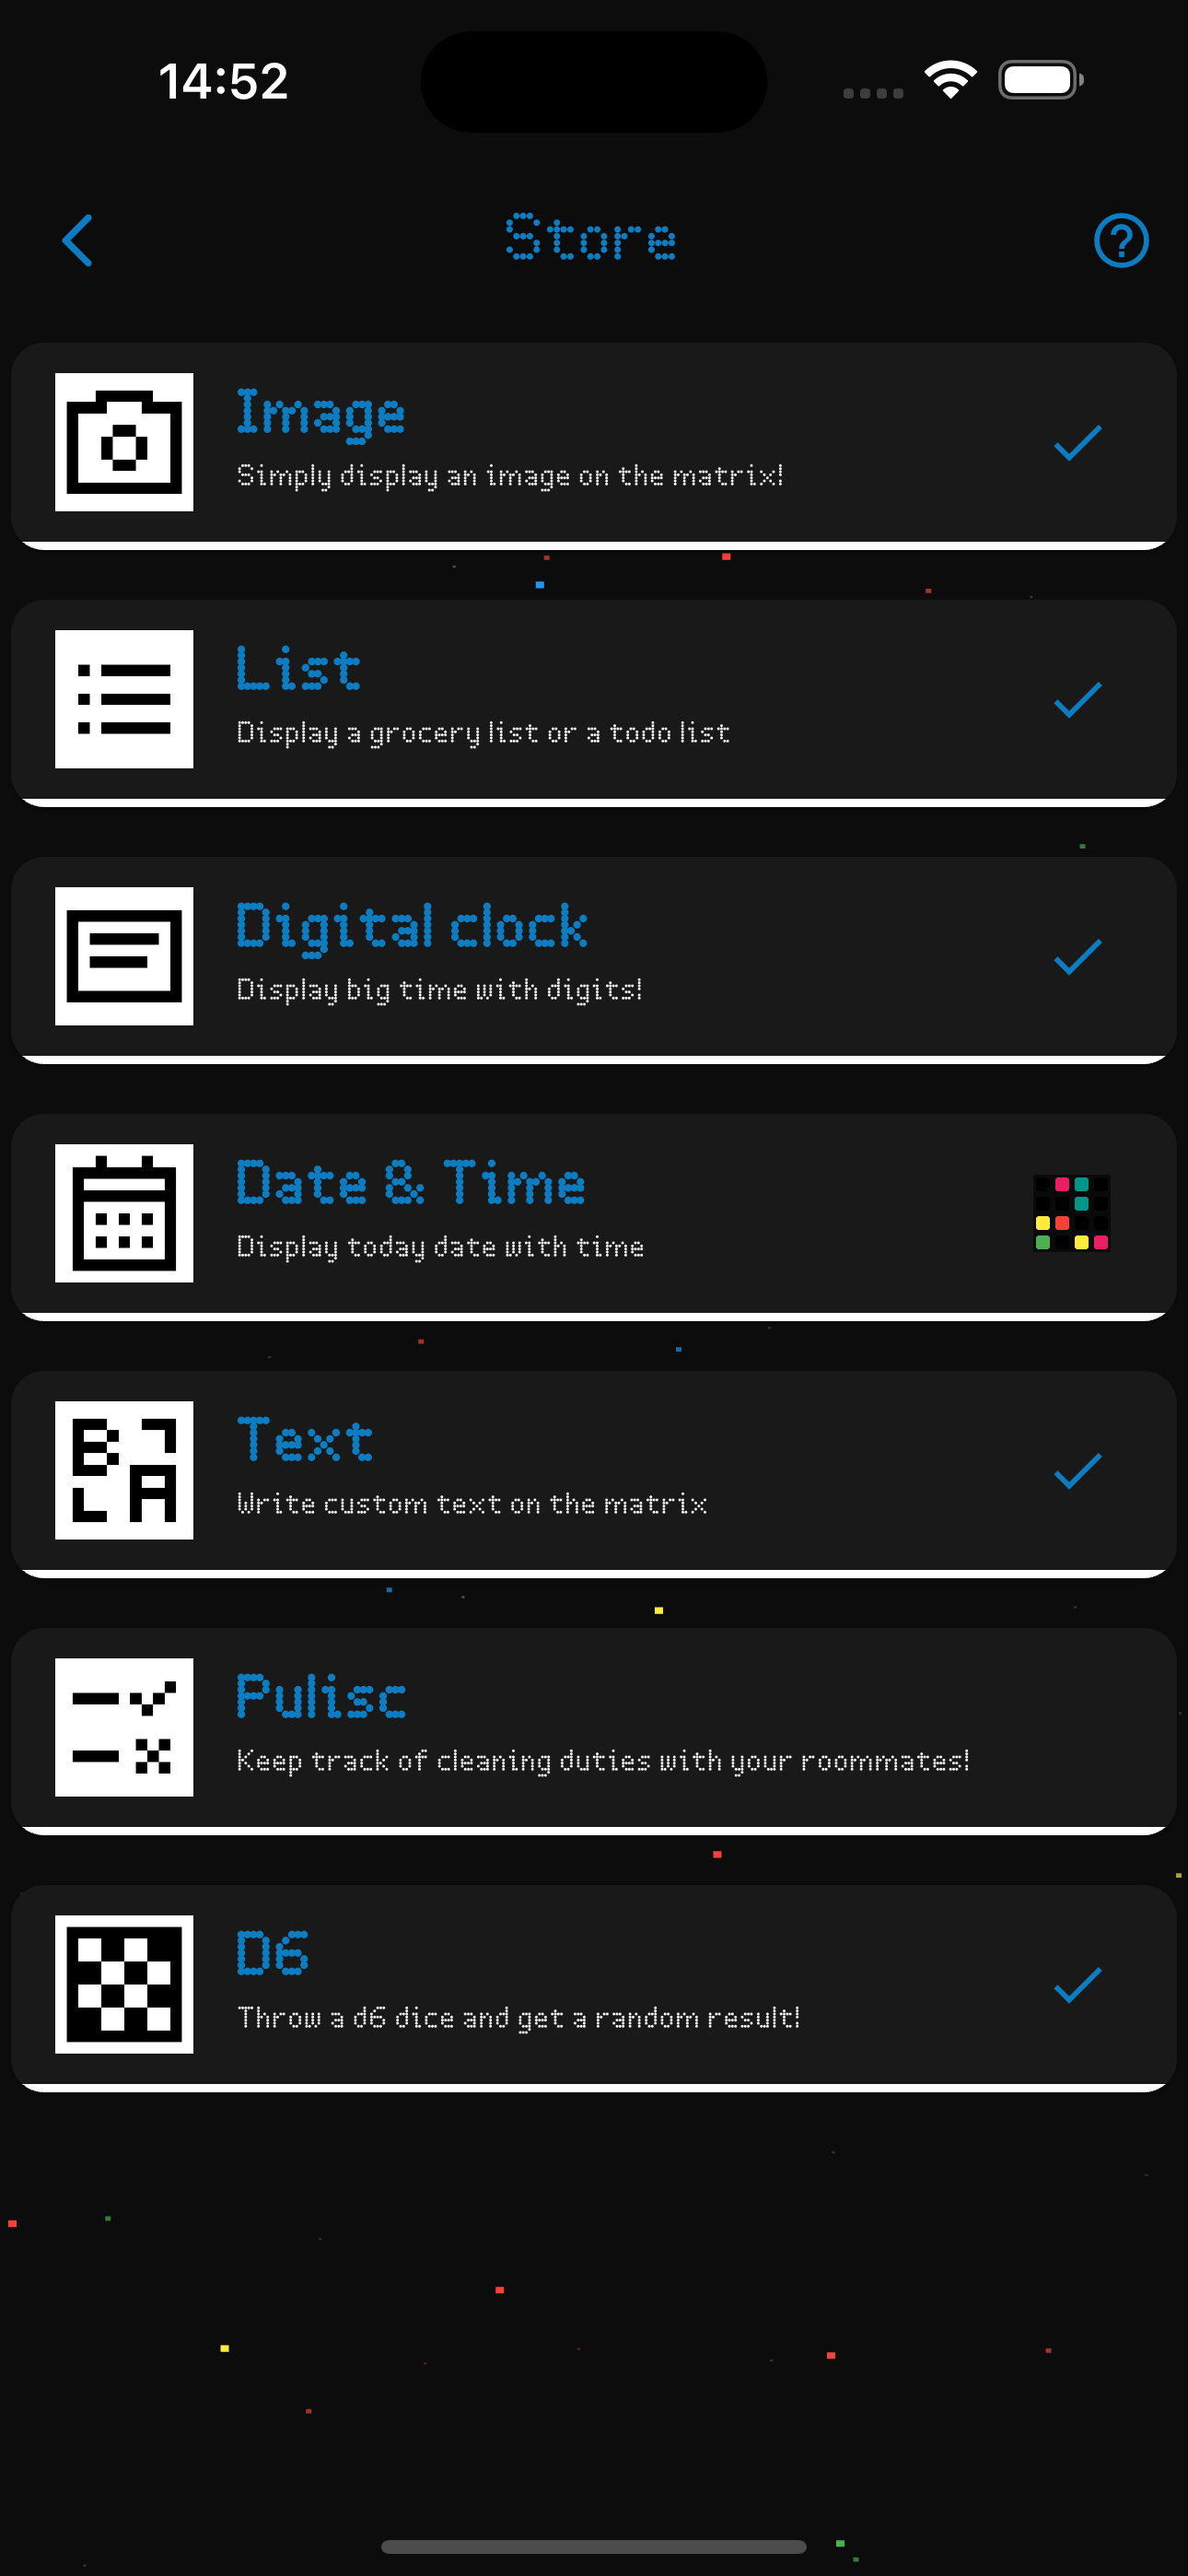
\includegraphics[width=\textwidth]{tesi/img/client_demo/store/widget_installing.png}
        \caption*{Installing a Widget}
    \end{minipage}
    \begin{minipage}[b]{0.32\textwidth}
        \centering
        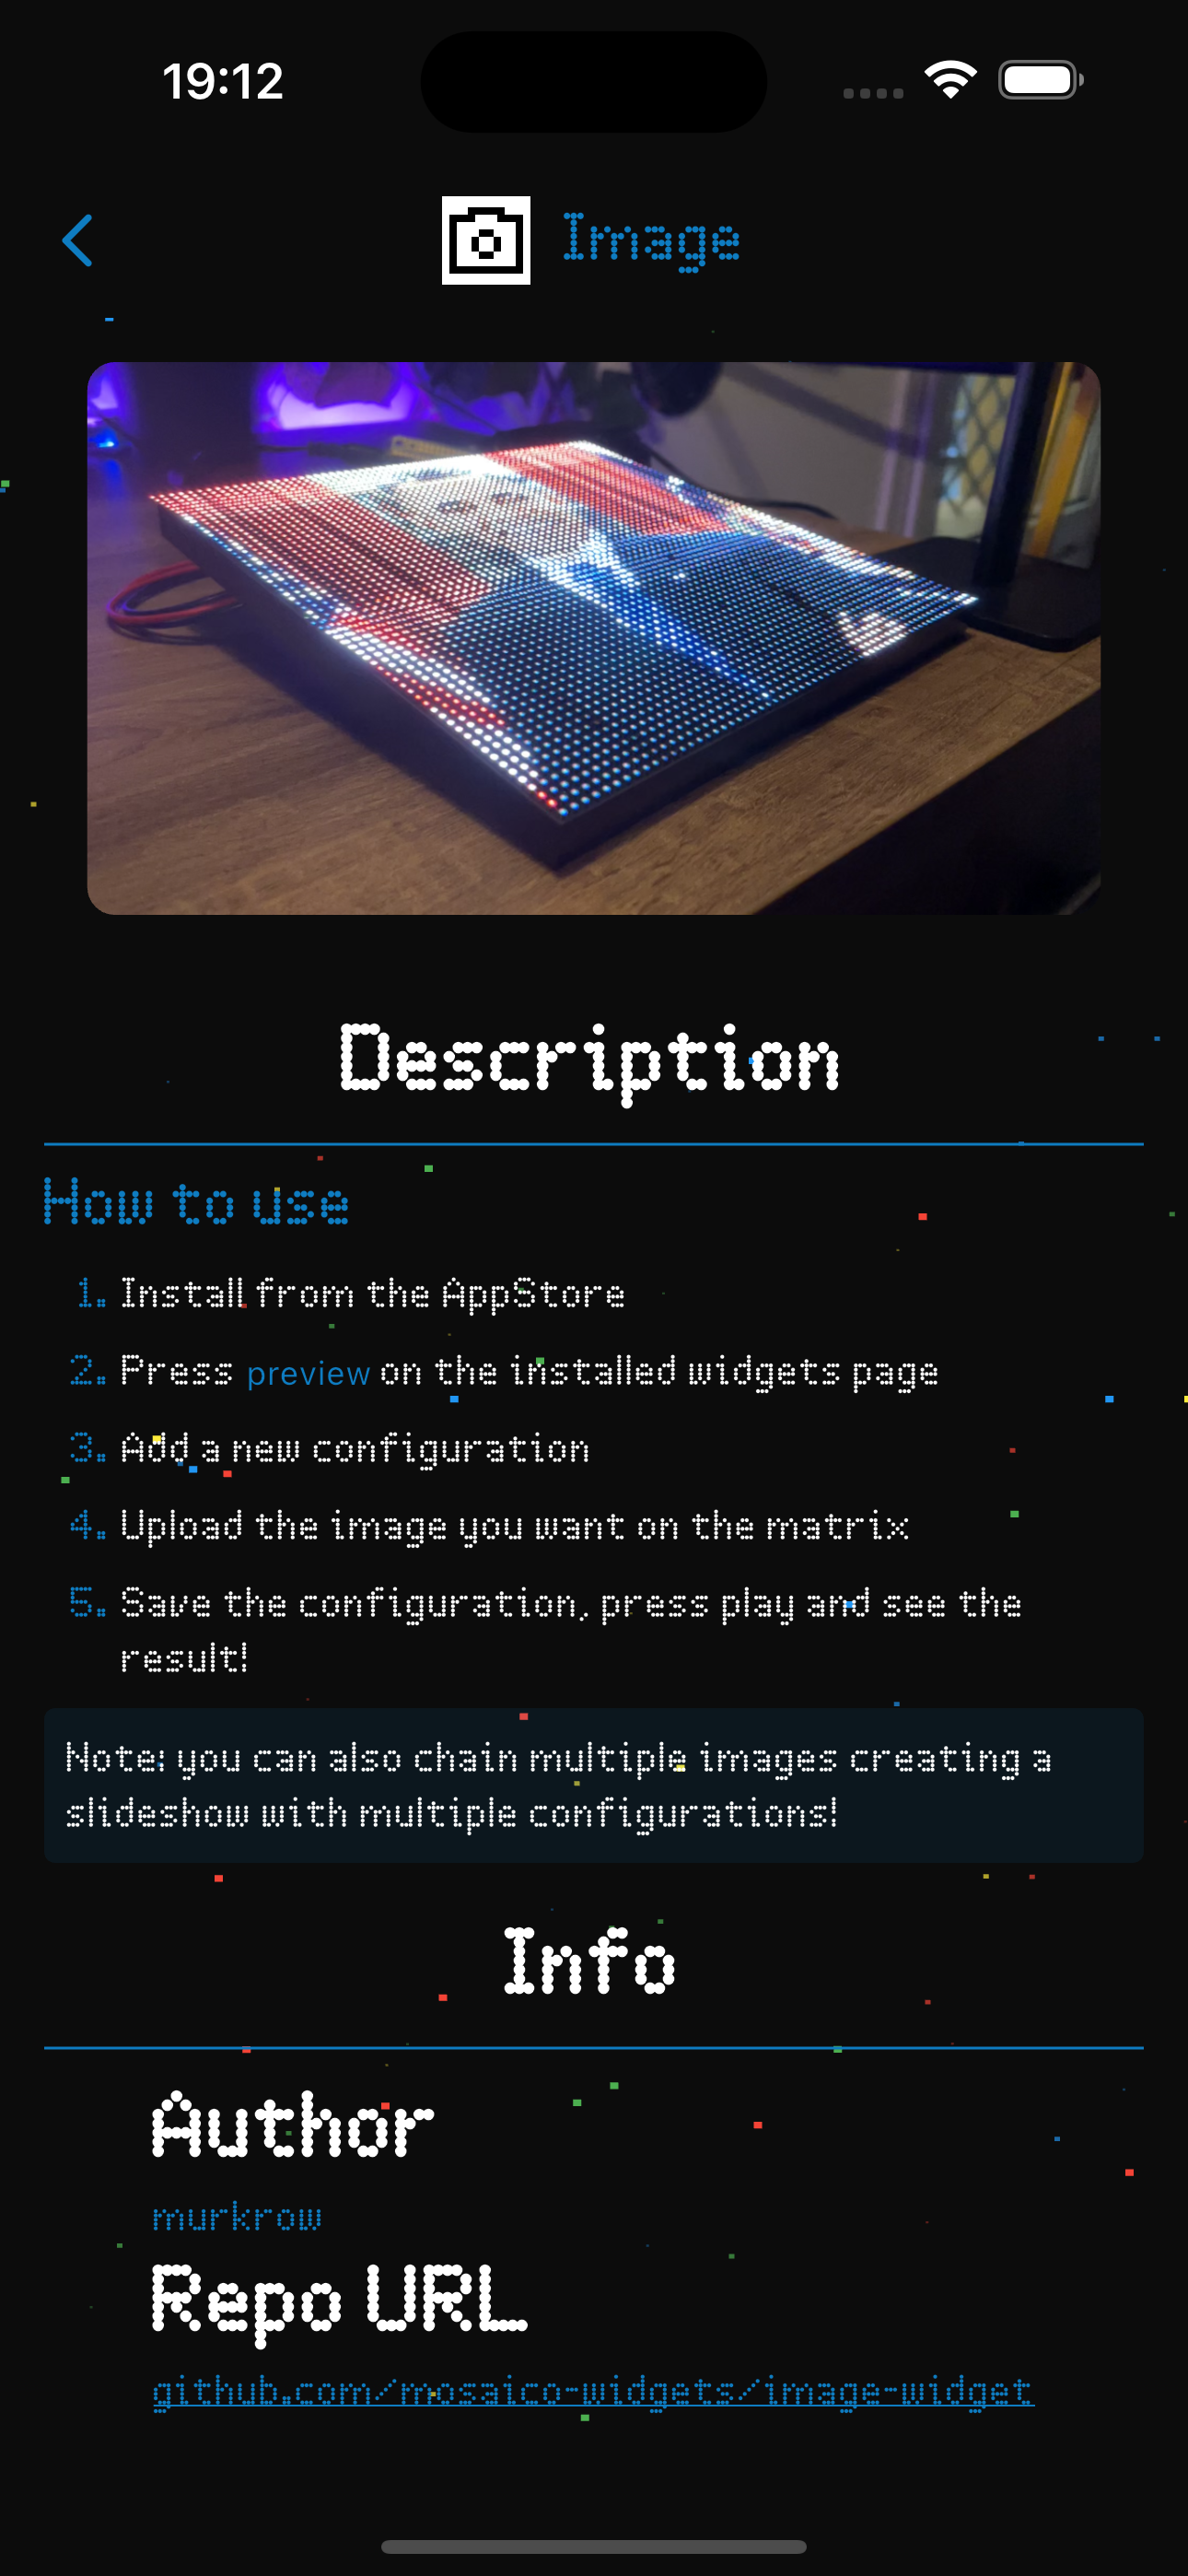
\includegraphics[width=\textwidth]{tesi/img/client_demo/store.png}
        \caption*{Widget Details}
    \end{minipage}
\end{figure}

\subsection{Slideshows}
Slideshows are sequences of widgets displayed consecutively on the matrix. This feature is particularly useful when users prefer to cycle through multiple widgets rather than display a single one continuously.

Creating a new slideshow is intuitive. Users are presented with cards containing two fields: a widget selector and a duration field where they can input the display time in seconds. If the selected widget is configurable, a third field will appear, allowing users to select a specific configuration for that item.

A floating action button in the bottom-right corner expands to provide three actions:
\begin{itemize}
    \item \textbf{Plus Icon}: Adds a new slideshow item card.
    \item \textbf{Save Icon}: Saves the current slideshow or creates a new one.
    \item \textbf{Play Icon}: Saves and immediately plays the current slideshow on the matrix.
\end{itemize}

\begin{figure}[h]
    \centering
    \begin{minipage}[b]{0.32\textwidth}
        \centering
        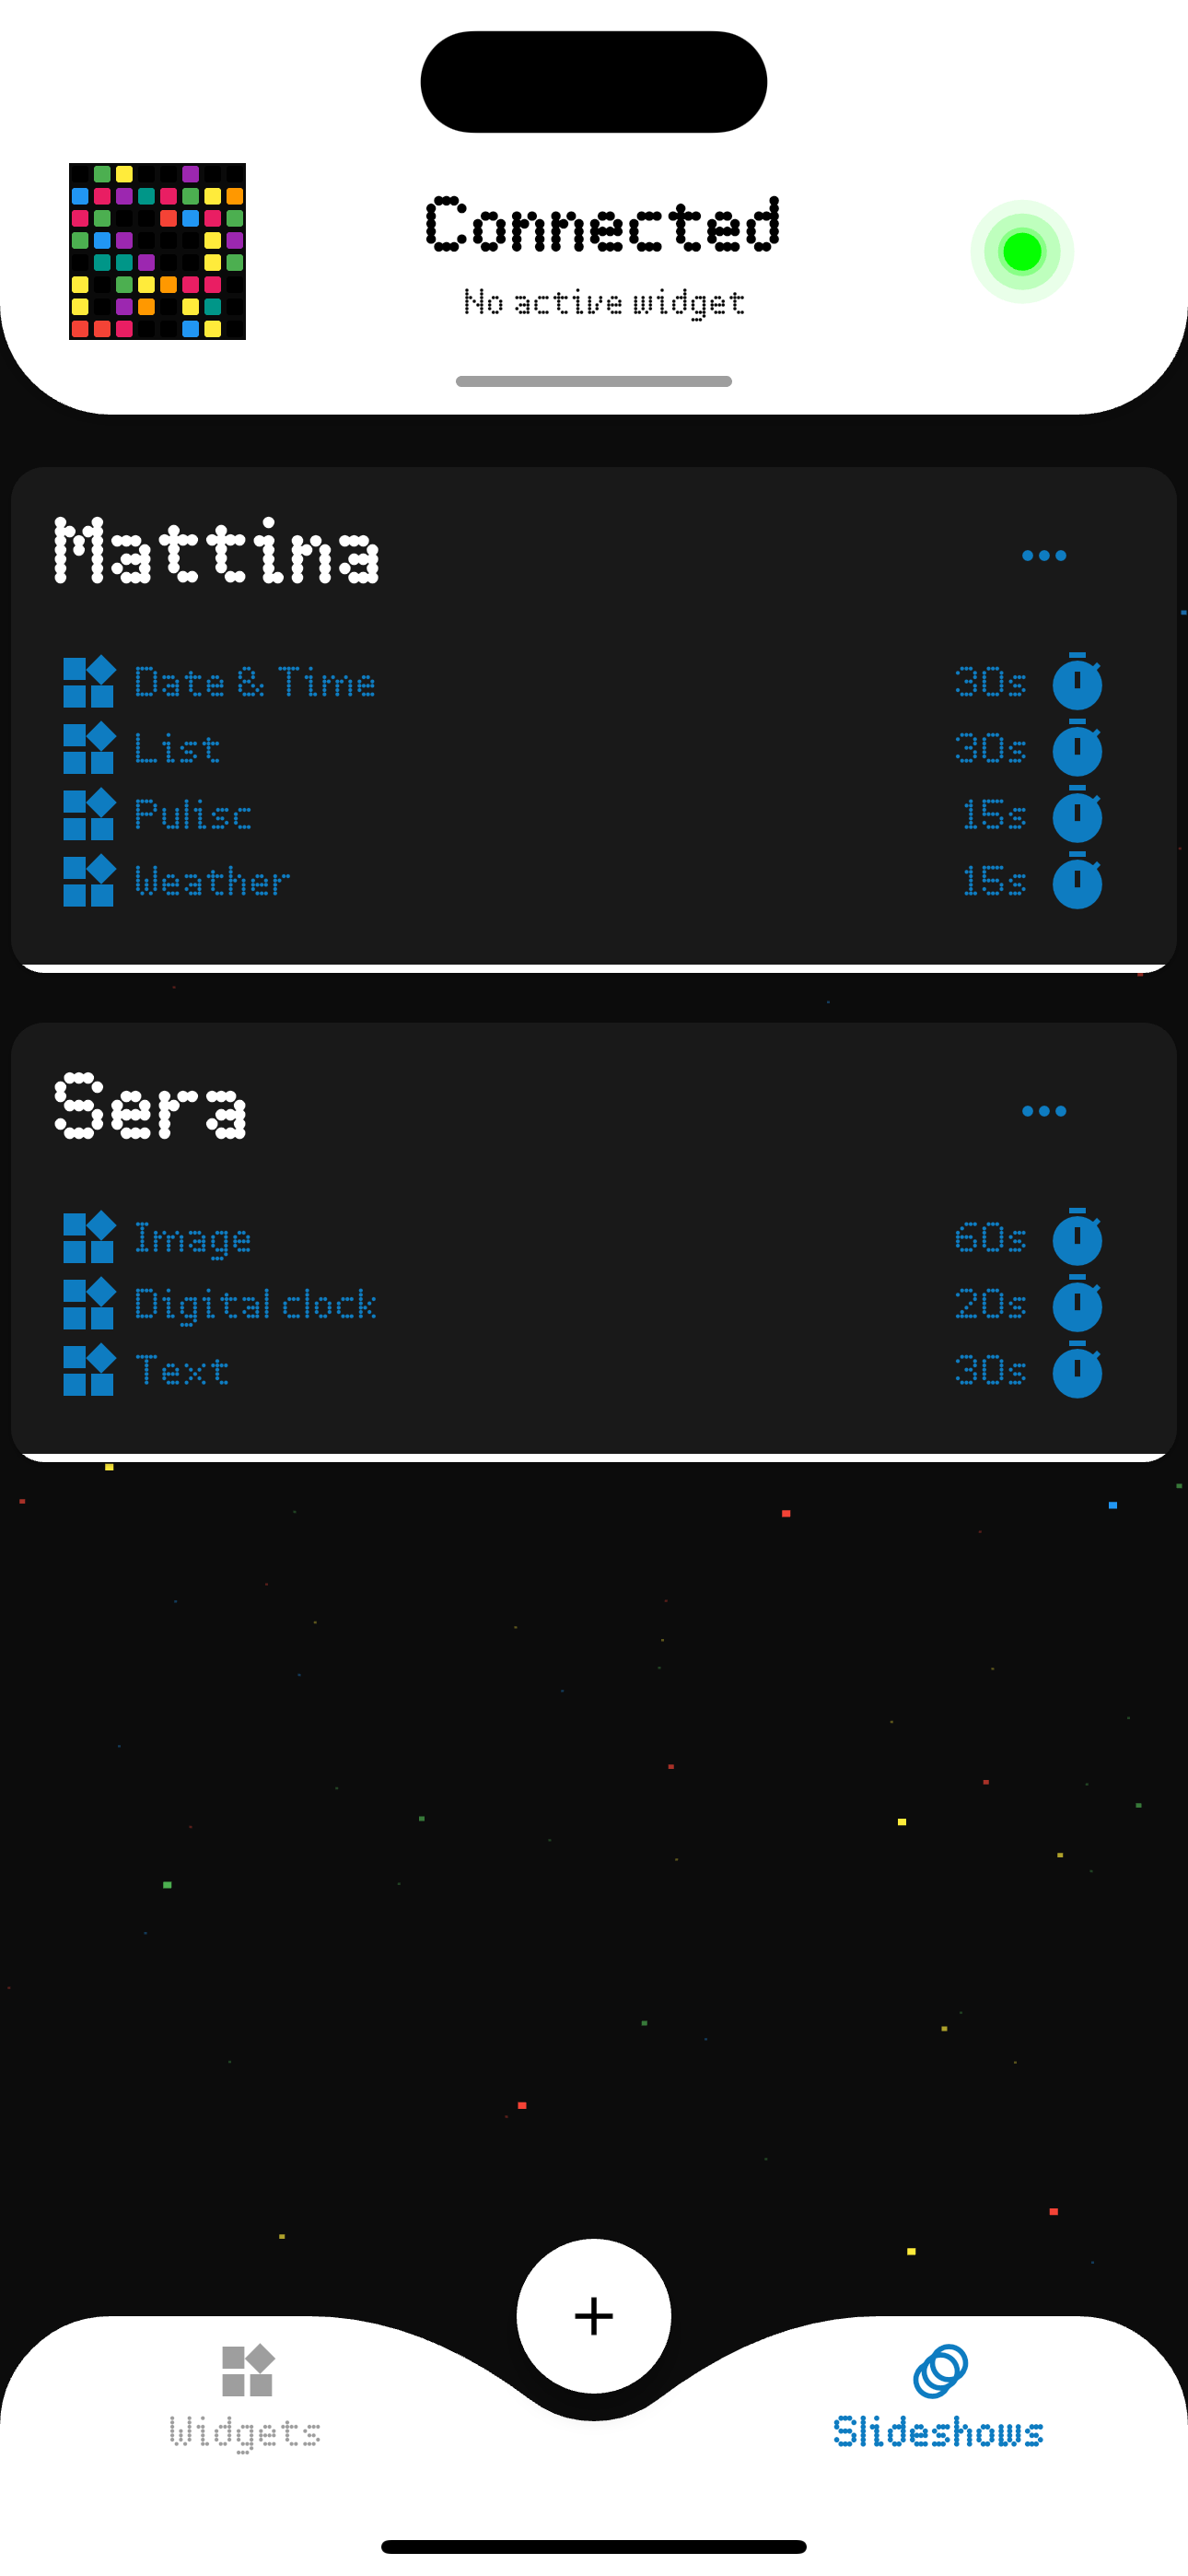
\includegraphics[width=\textwidth]{tesi/img/client_demo/slideshows/page.png}
        \caption*{Slideshows Page}
    \end{minipage}
    \begin{minipage}[b]{0.32\textwidth}
        \centering
        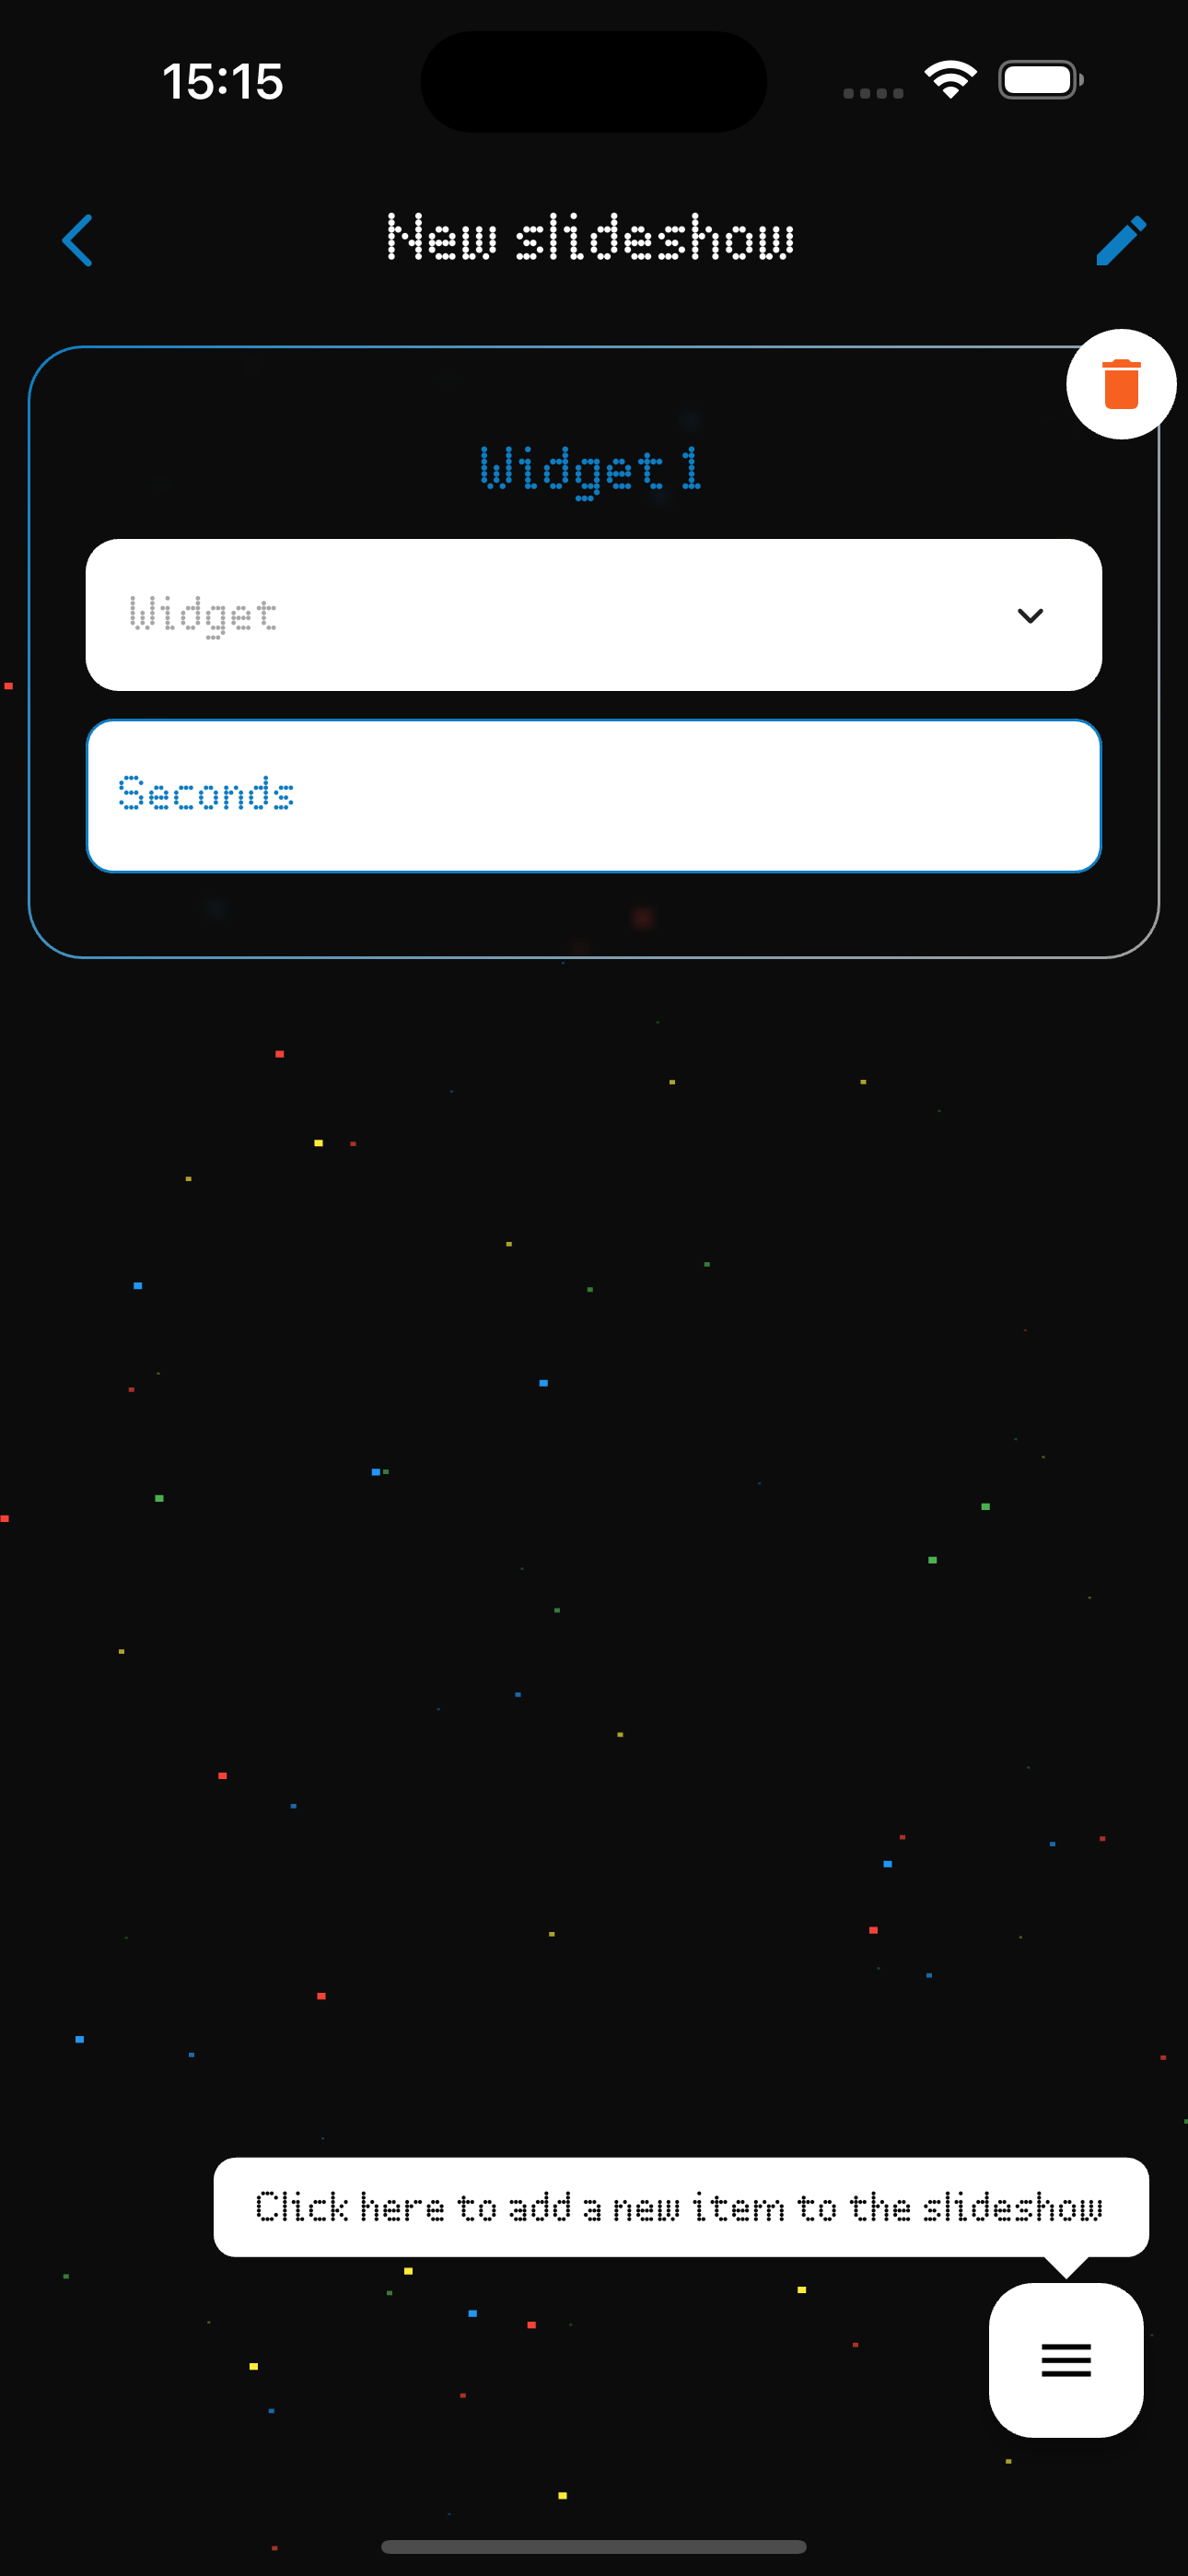
\includegraphics[width=\textwidth]{tesi/img/client_demo/slideshows/new.png}
        \caption*{Create a New Slideshow}
    \end{minipage}
    \begin{minipage}[b]{0.32\textwidth}
        \centering
        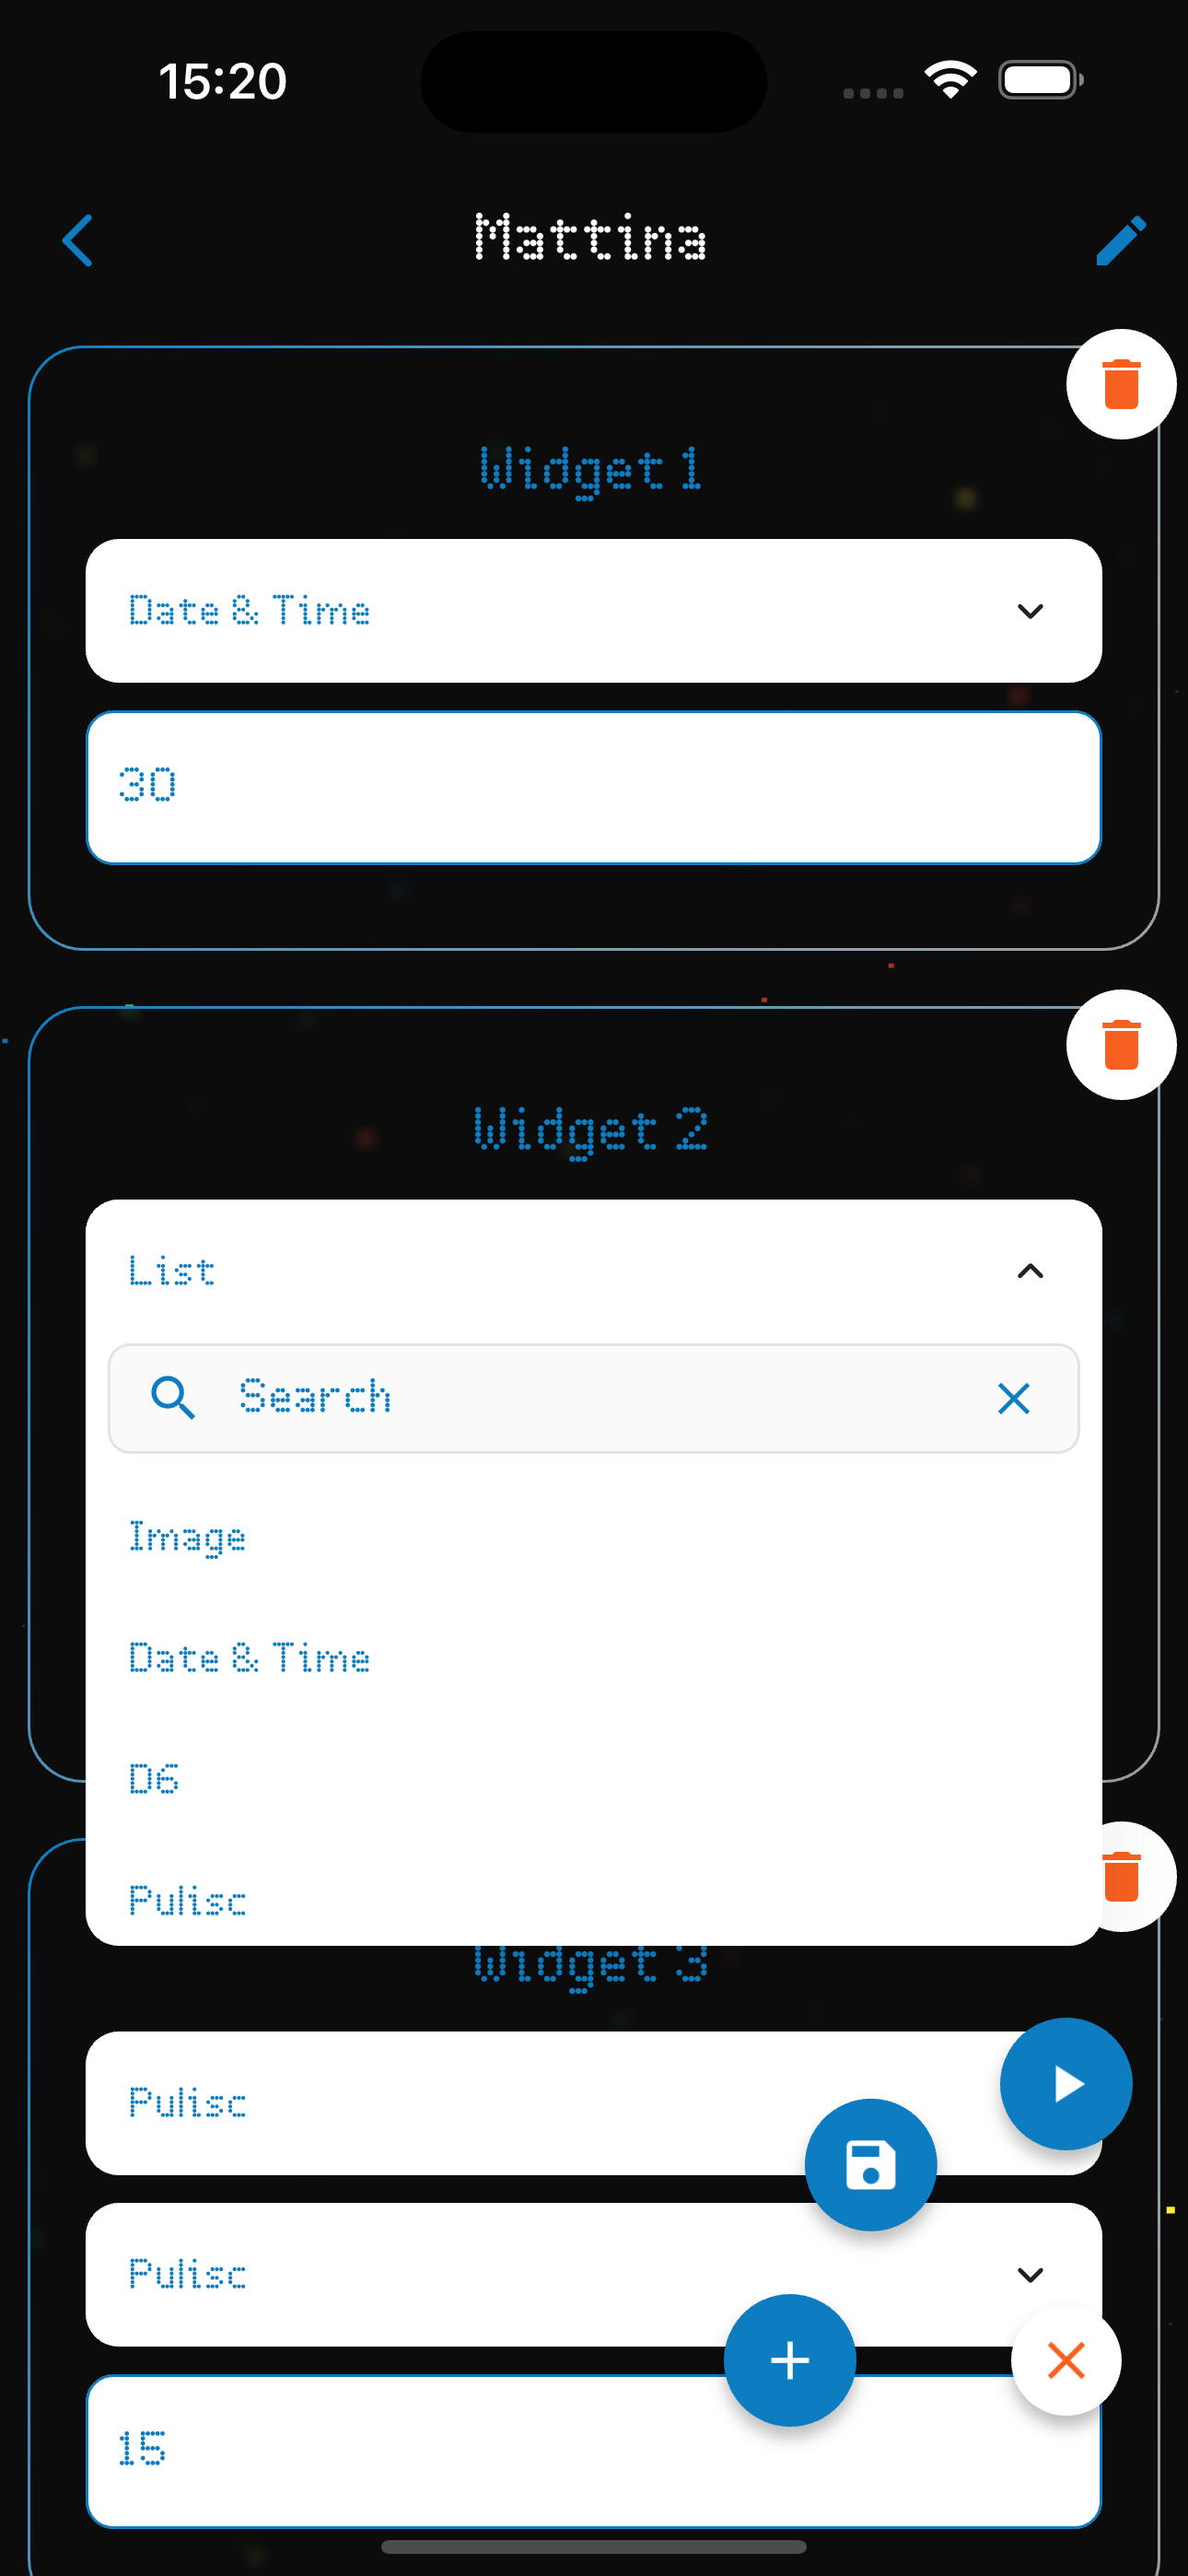
\includegraphics[width=\textwidth]{tesi/img/client_demo/slideshows/edit.png}
        \caption*{Edit an Existing Slideshow}
    \end{minipage}
\end{figure}

\section{Configuration Generator}
Configurable widgets \ref{widget-types} require a mechanism to collect data from users in order to configure the widget appropriately. 
Developers can create a configuration file in JSON format, which will be parsed by the configuration generator to dynamically create a form. 
This form allows the user to input the necessary data to configure the widget.

This design decision was crucial to ensuring that developers could create new widgets without needing to concern themselves with user interface design, while also maintaining consistency in the configuration process across widgets from different developers.

\subsection{Example}

A simple example of a configuration file to display a list of items is shown below:

\begin{minipage}{0.45\textwidth}
\begin{minted}{json}
{
  "form": {
    "title": "Shopping List",
    "description": "Configure your 
    widget here",
    "fields": [
      {
        "name": {
          "type": "string",
          "label": "Name",
          "required": true,
          "placeholder": "Enter the 
          name of this list"
        },
        "color": {
          "type": "color",
          "label": "Color",
          "required": true,
          "placeholder": "Choose the 
          color of the title"
        },
        "items": {
          "type": "string[]",
          "label": "Shopping items",
          "required": true,
          "placeholder": "Insert your 
          items here"
        }
      }
    ]
  }
}
\end{minted}
\end{minipage}
\hfill
\begin{minipage}{0.45\textwidth}
\centering
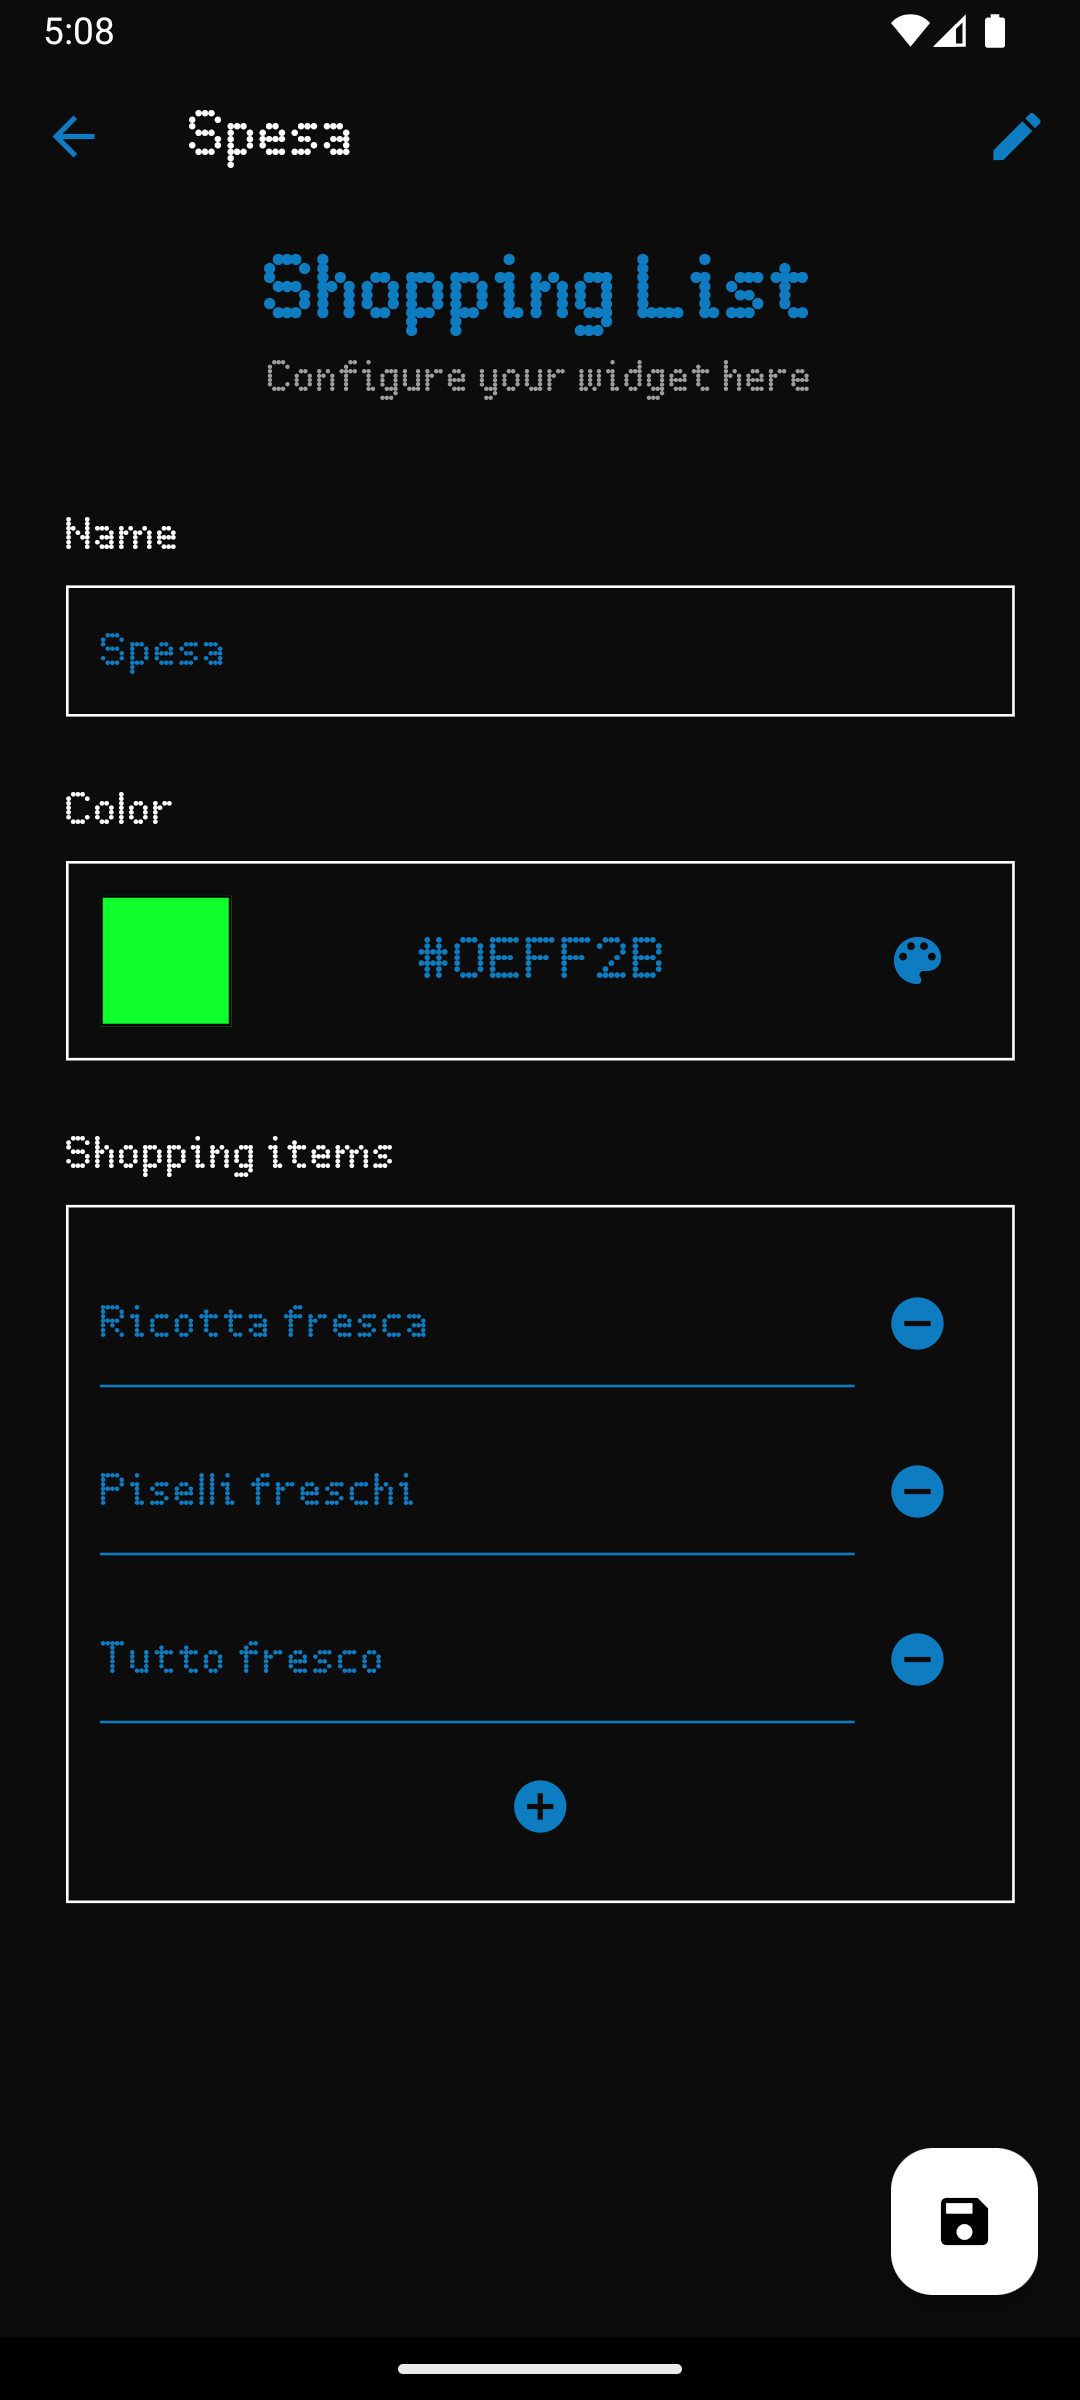
\includegraphics[width=\textwidth]{tesi/img/config_form/shopping_list_form.png}
\captionof{figure}{Client rendered form}
\end{minipage}

\subsection{Result of the Configuration}
The data collected from the user through the configuration form is saved in a JSON file. 
This file is parsed by the C++ engine when the specific widget with that configuration is loaded. 
Accessing the data from the configuration is straightforward in Python, as illustrated by the following example:

\begin{minipage}{0.65\textwidth}
\begin{minted}{python}
# config contains all the data from the configuration
from mosaico import widget, config

# Create title
text = widget.createText()
text.setText(config["name"])
text.setHexColor(config["color"])
text.moveTo(2,0)
text.setFont("9x18")

# Create items
items = []
bullets = []
for i in range(0, len(config["items"])):
    # Create bullet
    bullets.append(widget.createRectangle())
    bullets[i].setSize(2,2)        
    bullets[i].moveTo(4,16)
    bullets[i].translateYBy((i*7) + 5)    
    bullets[i].setHexColor(config["color"])  
    
    # Create entry  
    items.append(widget.createText())
    items[i].setFont("4x6")
    items[i].setText(config["items"][i])
    items[i].moveTo(8,14)    
    items[i].translateYBy((i*7) + 5)

def loop():
    pass
\end{minted}
\end{minipage}
\begin{minipage}{0.30\textwidth}
\centering
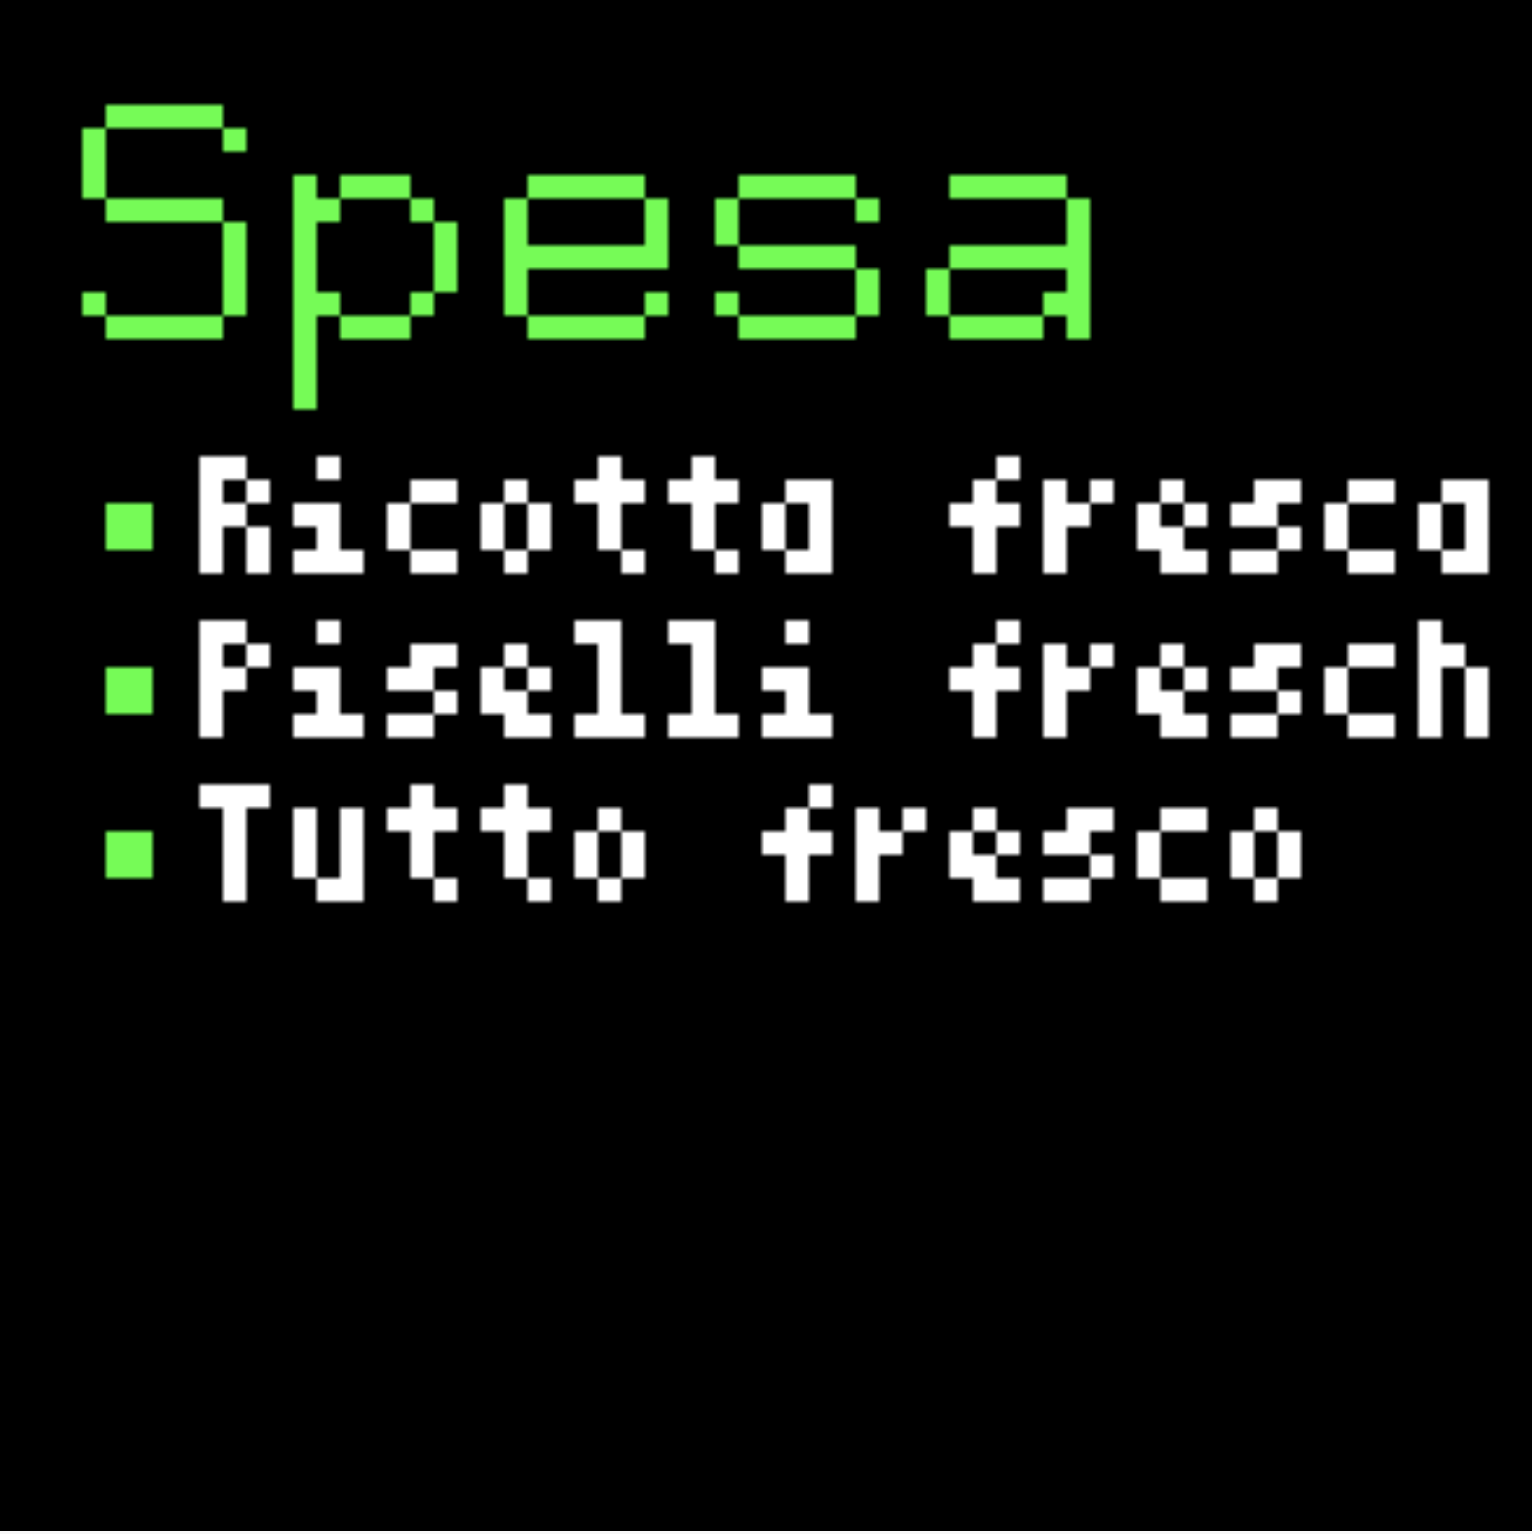
\includegraphics[width=\textwidth]{tesi/img/config_form/shopping_list_result.png}
\captionof{figure}{Result on matrix}
\end{minipage}

\subsection{Assets Management}
Each widget configuration is stored as a \texttt{.tar.gz} archive, which is essentially a compressed file that contains all the data submitted by the user. This compression facilitates faster transfers. Inside the archive, there is a \texttt{.json} file that holds the configuration details, as well as any additional binary files (e.g., images or other assets) uploaded by the user. A helper function is available to easily retrieve the path to these assets within the archive, simplifying access to the resources when needed.

\subsection{Field Attributes}
All fields share the following common attributes, regardless of their type:

\begin{itemize}
    \item \textbf{Name (required):} The unique identifier for the field within the configuration file. \textbf{Note:} \textit{You cannot use the same name for different fields}

    \item \textbf{Type (required):} Specifies the data type of the field. The type can be one of the following:
    \begin{itemize}
        \item \texttt{string}: A simple text field.
        \item \texttt{string[]}: An array of strings.
        \item \texttt{color}: A color picker field.
        \item \texttt{image}: An image upload field.
            \textbf{Special Attributes:}
            \begin{itemize}
            \item \texttt{Dimensions}: Specifies the image dimensions, as an object containing:
            \begin{itemize}
                \item \texttt{width}: The image width in pixels.
                \item \texttt{height}: The image height in pixels.
            \end{itemize}
            \end{itemize}
        \item \texttt{select}: An font selector between one of the available.
        \textbf{Special Attributes:}
            \begin{itemize}
            \item \texttt{options}: An array of strings, one will be selected by the user
            \end{itemize}
        \item \texttt{font}: An font selector between one of the available.
    \end{itemize}

    \item \textbf{Label:} The label displayed to the user in the configuration form to help them understand the purpose of the field.

    \item \textbf{Required:} A boolean value that indicates whether the field is mandatory.

    \item \textbf{Placeholder:} A placeholder text shown when the field is empty, providing guidance to the user about what to enter.
\end{itemize}


\subsection{Multiple configurations}
Obviously it would not make sense to create a configuration for one use only, once a configuration for a specific widget is created and user gave it a name, it will always be possible for them to list all the created, delete them or edit them using the appropriate 

\section{Device Discovery}
One of the essential features of the application is the automatic discovery mechanism, enabling seamless connectivity to a matrix device without requiring complex setup or manual configuration. The goal is to ensure that the application can autonomously identify and connect to any available matrix nearby.

Communication with the matrix device is handled through CoAP. However, in order to initiate this communication, the application must first obtain the IP address of the Raspberry Pi hosting the matrix. To address this challenge, a BLE GATT server is set up alongside the CoAP server. The GATT server exposes a service named \textit{Mosaico}, identified by a constant UUID, which the application can use to recognize the presence of a matrix. A simple BLE scan allows the application to detect this service and establish a connection.

The following algorithm outlines the process for automatically discovering and connecting to a matrix:

\begin{algorithm} \caption{Device discovery}\label{alg
} \begin{algorithmic} \Ensure Returns the matrix IP if successfully pinged, or \texttt{null} if all attempts fail

\State $prefs \gets \text{get preferences instance}$ \State $lastKnownMatrixIp \gets \text{get stored value from prefs}$ \If{$lastKnownMatrixIp \neq null$ \textbf{and} \texttt{pingMatrix}($lastKnownMatrixIp$)} \State \Return $lastKnownMatrixIp$ \EndIf

\If{\texttt{not} BLEDeviceConnected()} \State \texttt{searchAndConnectBleDevice()} \Comment{Attempt BLE connection} \EndIf

\State \texttt{ensureBleDeviceConnected()} \State $ipFromBle \gets \texttt{matrixBleService.getMatrixIp()}$ \If{$ipFromBle \neq null$ \textbf{and} \texttt{pingMatrix}($ipFromBle$)} \State \texttt{prefs.setString('matrixIp', ipFromBle)} \State \Return $ipFromBle$ \EndIf

\State \Return \texttt{null} \end{algorithmic} \end{algorithm}

If the automatic discovery process is unsuccessful, users can manually set the matrix IP address via the \textit{Set Manual Matrix Address} option in the device control panel, allowing them to connect to the matrix manually.

\section{Caching}
The constrained capabilities of the Raspberry Pi Zero W represent the primary limitation in the Mosaico ecosystem. While its core function is to render dynamic content on the LED matrix, it also operates as both a COAP and BLE server, facilitating communication with the mobile application. The dual responsibilities placed on the Pi necessitate careful management of system resources to avoid overburdening the device, particularly when handling frequent network requests.

To mitigate unnecessary strain on the Raspberry Pi, Mosaico employs efficient caching mechanisms within the mobile client. This reduces redundant calls to the COAP server, especially for frequently accessed data such as installed widgets, created slideshows, and widget configurations. The caching strategy is straightforward yet effective: commonly requested services are retrieved once, typically when users initially open the app or navigate to specific sections that trigger those requests. Subsequent interactions with these services do not require re-querying the COAP server unless there is a change, such as the installation of a new widget. In such cases, the cache is intelligently updated in memory without fully refreshing the entire dataset.

The use of caching not only improves the user experience by speeding up interactions but also reduces the overall communication overhead on the Raspberry Pi, ensuring that its limited resources are efficiently utilized. By implementing an in-memory cache for frequently accessed data, Mosaico reduces the need for repetitive data fetching, which would otherwise place undue load on the system. This approach ensures the platform remains responsive, even on the resource-constrained Raspberry Pi Zero W.

From a broader perspective, this resource-conscious design exemplifies how careful consideration of hardware limitations can be balanced with software optimizations to maintain system performance. By integrating caching strategies, Mosaico achieves a more scalable solution while prolonging the lifespan and effectiveness of the hardware within the IOT ecosystem.

\section{Design Patterns}
In the mobile application development of Mosaico, the \textbf{BLoC (Business Logic Component)} design pattern was utilized to manage and maintain the app's state in a scalable and organized manner. The separation of concerns provided by BLoC ensures that the UI reacts to changes in the app's state efficiently, promoting cleaner, testable, and maintainable code.

BLoC acts as the intermediary between the UI and the business logic of the application, where each BLoC listens to \textbf{events} and emits corresponding \textbf{states}. This makes it ideal for applications where user interactions and changes in data need to be reflected dynamically across different parts of the UI.

\subsection{BLoC for Installed Widgets Feature}

An excellent example of BLoC in action can be seen in the \textbf{Installed Widgets Page}. This page showcases widgets that users have installed on their LED matrix devices. Using a combination of \textbf{BlocListeners} and \textbf{BlocBuilders}, the UI dynamically updates based on external events such as matrix connections or widget store interactions.

\begin{minted}{dart}
return MultiBlocListener(
  listeners: [
    BlocListener<MatrixDeviceBloc, MatrixDeviceState>(
      listener: (context, state) {
        // Only refresh installed widgets if connected to a new matrix
        if (state is MatrixDeviceConnectedState && state.newConnection) {
          context.read<MosaicoInstalledWidgetsBloc>()
              .add(LoadInstalledWidgetsEvent());
        }
      },
    ),
    BlocListener<MosaicoStoreBloc, MosaicoStoreState>(
      listener: (context, state) {
        // Refresh when new widgets are available from the store
        if (state is MosaicoStoreLoadedState) {
          context.read<MosaicoInstalledWidgetsBloc>()
              .add(LoadInstalledWidgetsEvent());
        }
      },
    ),
  ],
  child: BlocBuilder<MosaicoInstalledWidgetsBloc, MosaicoInstalledWidgetsState>(
    builder: (context, state) {
          // Handle different states (Loading, Loaded, Error)
          // and provide the appropriate UI response.
          
          // Loading
          if (state is MosaicoInstalledWidgetsLoading) {
            return Center(child: Center(child: LoadingMatrix()));
          }

          // Loaded
          if (state is MosaicoInstalledWidgetsLoaded) {
           if (state.installedWidgets.isEmpty) {
              return const EmptyPlaceholder(
                  hintText: "No widgets? Install some from the store!");
            }
            // Show installed widgets tiles
          }

          // Error
          if (state is MosaicoInstalledWidgetsError) {
            return EmptyPlaceholder(
              hintText: state.message,
              onRetry: () {
                context
                    .read<MosaicoInstalledWidgetsBloc>()
                    .add(LoadInstalledWidgetsEvent());
              },
            );
          }

          // Not connected?
          return const EmptyPlaceholder(
              hintText: "Connect to matrix to see installed widgets");
    },
  ),
);
\end{minted}

In this code, the \textbf{InstalledWidgetsPage} listens for events from multiple BLoCs:

\begin{itemize}
    \item \textbf{MatrixDeviceBloc} triggers updates when a new connection is made to an LED matrix device.
    \item \textbf{MosaicoStoreBloc} listens for changes in the widget store, refreshing the installed widgets list when new widgets are available for installation.
\end{itemize}

This dynamic reaction between BLoCs allows different parts of the app to remain in sync, minimizing redundant requests and ensuring that data is updated only when necessary.

\subsection{BLoC for Widget Store Interactions}

In the \textbf{Mosaico Store}, when a user installs a new widget, the \textbf{MosaicoStoreBloc} processes this event by calling the appropriate repository to handle the widget installation. Once completed, the store emits an updated state that is listened to by other components, like the \textbf{Installed Widgets Page}, so the newly installed widget appears without additional user action.

This interaction emphasizes the power of BLoC to coordinate state changes across different sections of the app. When a new widget is installed, the state is updated across all relevant UI components in real-time.

By employing the BLoC pattern, the app benefits from a well-structured and responsive design where state changes in one area, such as the widget store, can immediately reflect in another, like the list of installed widgets. This approach reduces unnecessary API calls and ensures the app provides an efficient user experience.

This section highlights the practical advantages of the BLoC pattern, reinforcing its role in handling complex state management tasks in a clean and modular way.